\chapter{QuantMAC-VO: Quantization for Learning-Based Visual Odometry with Metrics-Aware Covariance} \label{chapter:quantmacvo}
\fancyhead[LO]{\makebox[\textwidth][r]{Chapter 4. QuantMAC-VO}}

\section{Introduction}
\label{sec:quantmacvo_intro}

Recently, learning-based Visual Odometry (VO)~\cite{wang2017deepvo, li2018undeepvo,wang2021tartanvo,dpvo,qiu2025mac} has emerged as a robust paradigm for state estimation in robotics, outperforming traditional geometric methods in challenging dynamic and texture-poor environments~\cite{mur2015orb,mur2017orb,campos2021orb}. However, this performance gain comes with heavy computational and memory demands, making such models prohibitive for deployment on resource-constrained edge platforms.

Model quantization~\cite{nagel2021white,krishnamoorthi2018quantizing}, particularly Post-Training Quantization (PTQ), has become the \textit{de facto} standard for efficient deployment of deep neural networks~\cite{zhoulidar,ptq4vit,frantar2022gptq,xiao2022smoothquant}. 
However, most PTQ methods rely on a small calibration dataset and implicitly assume that its activation statistics are representative of deployment conditions. 
This assumption breaks down for learning-based VO, where long-horizon motion dynamics, viewpoint changes, and scene-dependent geometry induce highly non-stationary and heavy-tailed activations. 
As a result, quantization parameters calibrated on limited sequences tend to overfit to specific environments and fail to generalize, leading to significant performance degradation when deployed on robots operating in previously unseen real-world scenarios.

In addition, learning-based VO networks exhibit pronounced heavy-tailed activations and spatially localized outliers as shown in \fref{fig:spatial_outlier}, which significantly hinder effective quantization. 
To address this, Hadamard rotation~\cite{ashkboos2024quarot} has been proposed to disperse outliers across dimensions via an orthogonal transform, thereby improving quantization robustness. 
However, this strategy introduces new challenges in the context of learning-based odometry. 
VO architectures typically consist of many layers with relatively small feature dimensions, for which the computational and memory overhead of applying Hadamard rotations becomes non-negligible. 
When deployed on edge platforms, the added cost of these rotations can dominate inference time, and in some cases, even result in slower execution than the unquantized model.

To address these challenges, this chapter presents a full-stack quantization framework for learning-based VO with metrics-aware covariance, built upon MAC-VO (Chapter~\ref{chapter:macvo}) and a foundation calibration dataset grounded in TartanAir~\cite{tartanair}. 
Inspired by the strong sim-to-real transferability of visual foundation models and modern learning-based VO systems~\cite{qiu2025mac}, we leverage a large-scale, diverse calibration source to improve quantization robustness across environments. 
To mitigate the computational overhead introduced by rotation-based quantization, we propose a kurtosis-based hybrid quantization strategy that selectively applies computationally expensive online rotations only to critical layers exhibiting spatial outliers, while employing efficient offline channel smoothing for channel-wise outliers. 
Beyond frontend acceleration, we further investigate quantization effects in the backend pose optimization.
We find that applying the scaling factor to the Gauss-Newton optimizer is mathematically equivalent to scaling the coordinate of the pose estimation.
Therefore, our quantization on the back-end optimizer maintains consistent performance.
As shown in \fref{fig:teasear}, we deployed the proposed system on the NVIDIA Jetson Thor edge platform, demonstrating real-time performance with negligible accuracy loss on resource-constrained robotic hardware. 
The main contributions of this chapter are:

\begin{itemize} 
\item We introduce a sim-to-real quantization calibration strategy enabling zero-shot generalization without re-calibration, and observe a scaling law whereby real-world performance improves monotonically with the diversity of synthetic calibration data.

\item We propose a {kurtosis-based hybrid quantization} method that selectively applies Hadamard rotations to layers with high kurtosis, reducing system overhead while maintaining high quantization efficiency.

\item We investigate backend optimization under quantization by introducing explicit scaling factors, and show that the resulting formulation is mathematically equivalent to solving pose estimation under a scaled coordinate system.

\item We demonstrate that the proposed quantization framework accelerates MAC-VO by 1.83$\times$ on the NVIDIA Jetson Thor platform, achieving real-time performance with negligible accuracy degradation.

\end{itemize}

\begin{figure}[t]
  \centering
  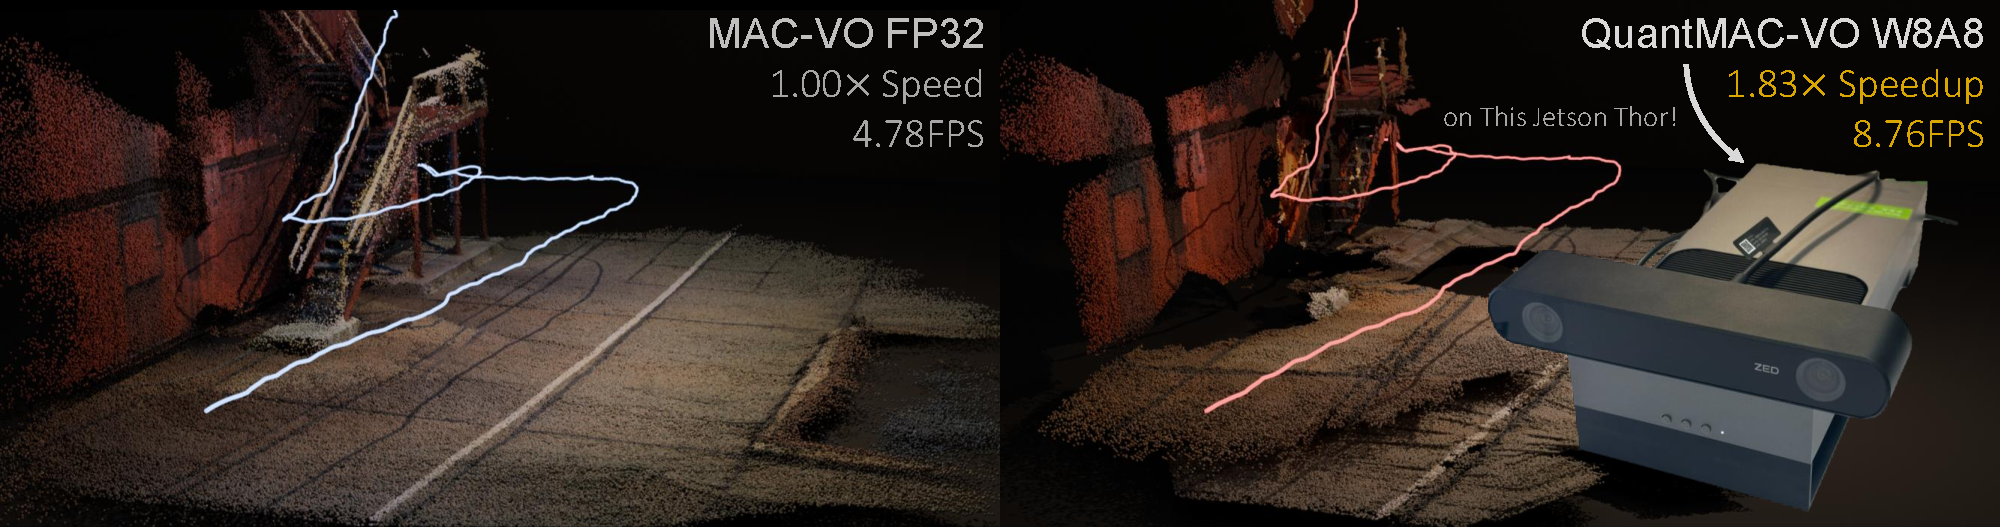
\includegraphics[width=1\linewidth]{tex/ch4_quantmacvo/figs/Fig1-QuantMACVO.pdf}
  \captionsetup{font=small}
  \caption{QuantMAC-VO deployed on the NVIDIA Jetson Thor platform, achieving real-time learning-based visual odometry with metrics-aware covariance on edge hardware.}
  \label{fig:teasear}
\end{figure}


\section{Related Work}
\label{sec:quantmacvo_related}

\subsection{Quantization for Neural Networks}
\label{sec:quantization}

Existing post-training quantization (PTQ) methods are categorized into weight-only and weight-activation quantization~\citep{zhao2023survey}. Weight-only methods are commonly used for LLMs, like GPTQ~\citep{frantar2022gptq} and AWQ~\citep{lin2024awq}, which achieve high compression rates but offer limited inference acceleration. In contrast, weight-activation quantization methods~\citep{xiao2022smoothquant, yuan2023asvd} quantize both weights and activations, improving memory usage and latency. The main challenge is activation outliers causing quantization errors. Techniques like SmoothQuant~\citep{xiao2022smoothquant} shift quantization difficulty from activations to weights, while OmniQuant~\citep{2023omniquant} optimizes performance by training quantization parameters. Recently, Quarot~\citep{ashkboos2024quarot} introduced rotations to eliminate outliers; however, this solution is not applicable to MLLMs due to inherent modality differences.

\subsection{Quantization for SLAM}
\label{sec:slam_quant}

Traditional geometric visual odometry systems primarily rely on minimizing reprojection or photometric errors \cite{mur2015orb, engel2014lsd}, typically employing fixed covariance heuristics that often falter in complex environmental dynamics. 
The advent of deep learning has fundamentally reshaped this landscape, delivering significant performance leaps in core components such as optical flow estimation \cite{teed2020raft, parameshwara2022diffposenet}, dense depth prediction \cite{li2018undeepvo, zhou2017unsupervised, zuo2021codevio, xin2023simplemapping}, and learnable feature matching \cite{sarlin2020superglue, wang2023dust3r}. 

Building upon these advancements, hybrid SLAM architectures have emerged to synergize the robustness of geometric constraints with the adaptability of data-driven priors \cite{yang2020d3vo, teed2021droid}. 
A critical innovation in these modern frameworks is the integration of learned uncertainty. 
Unlike earlier methods that utilized static empirical priors \cite{Javier2008InverseDepth}, recent approaches employ neural networks to predict pixel-wise confidence or depth covariance \cite{Dexheimer_2023_learndepthcov, Wannenwetsch_2017_ICCV}, which serve as dynamic weights during factor graph optimization or differentiable bundle adjustment \cite{teed2021droid, muhle2023learning}. Methods like QVIO~\cite{peng2024qvio, peng2025qvio2} focus on quantizing raw sensor measurements or residuals.
However, many existing systems, such as DROID-SLAM \cite{teed2021droid}, often resort to simplified diagonal covariance models, potentially neglecting scale consistency which is vital for rigorous sensor fusion. Based on this, SPAQ-DL-SLAM~\cite{pudasaini2024spaq} compresses DROID-SLAM by applying pruning and quantization strictly to the neural modules. However, they leave the backend untouched in high precision. Furthermore, the strategy for keypoint selection has evolved. While classical descriptors \cite{orb2011} and early learned extractors \cite{superpoint2018} predominantly target high-frequency regions like edges and corners, recent studies suggest that these areas are prone to interpolation artifacts and neural ambiguity, potentially degrading state estimation \cite{teed2024deep, yang2020d3vo}. 
Consequently, state-of-the-art frameworks (e.g., MAC-VO, Chapter~\ref{chapter:macvo}) utilize learned uncertainty maps to actively filter unreliable features, ensuring that only high-quality constraints enter the backend optimization. 
The increasing reliance on these sophisticated, heavy-weight uncertainty estimation networks underscores the necessity for efficient quantization strategies to facilitate their deployment on edge devices.


\section{Method}
\label{sec:quantmacvo_method}

\begin{figure*}[t]
  \centering
  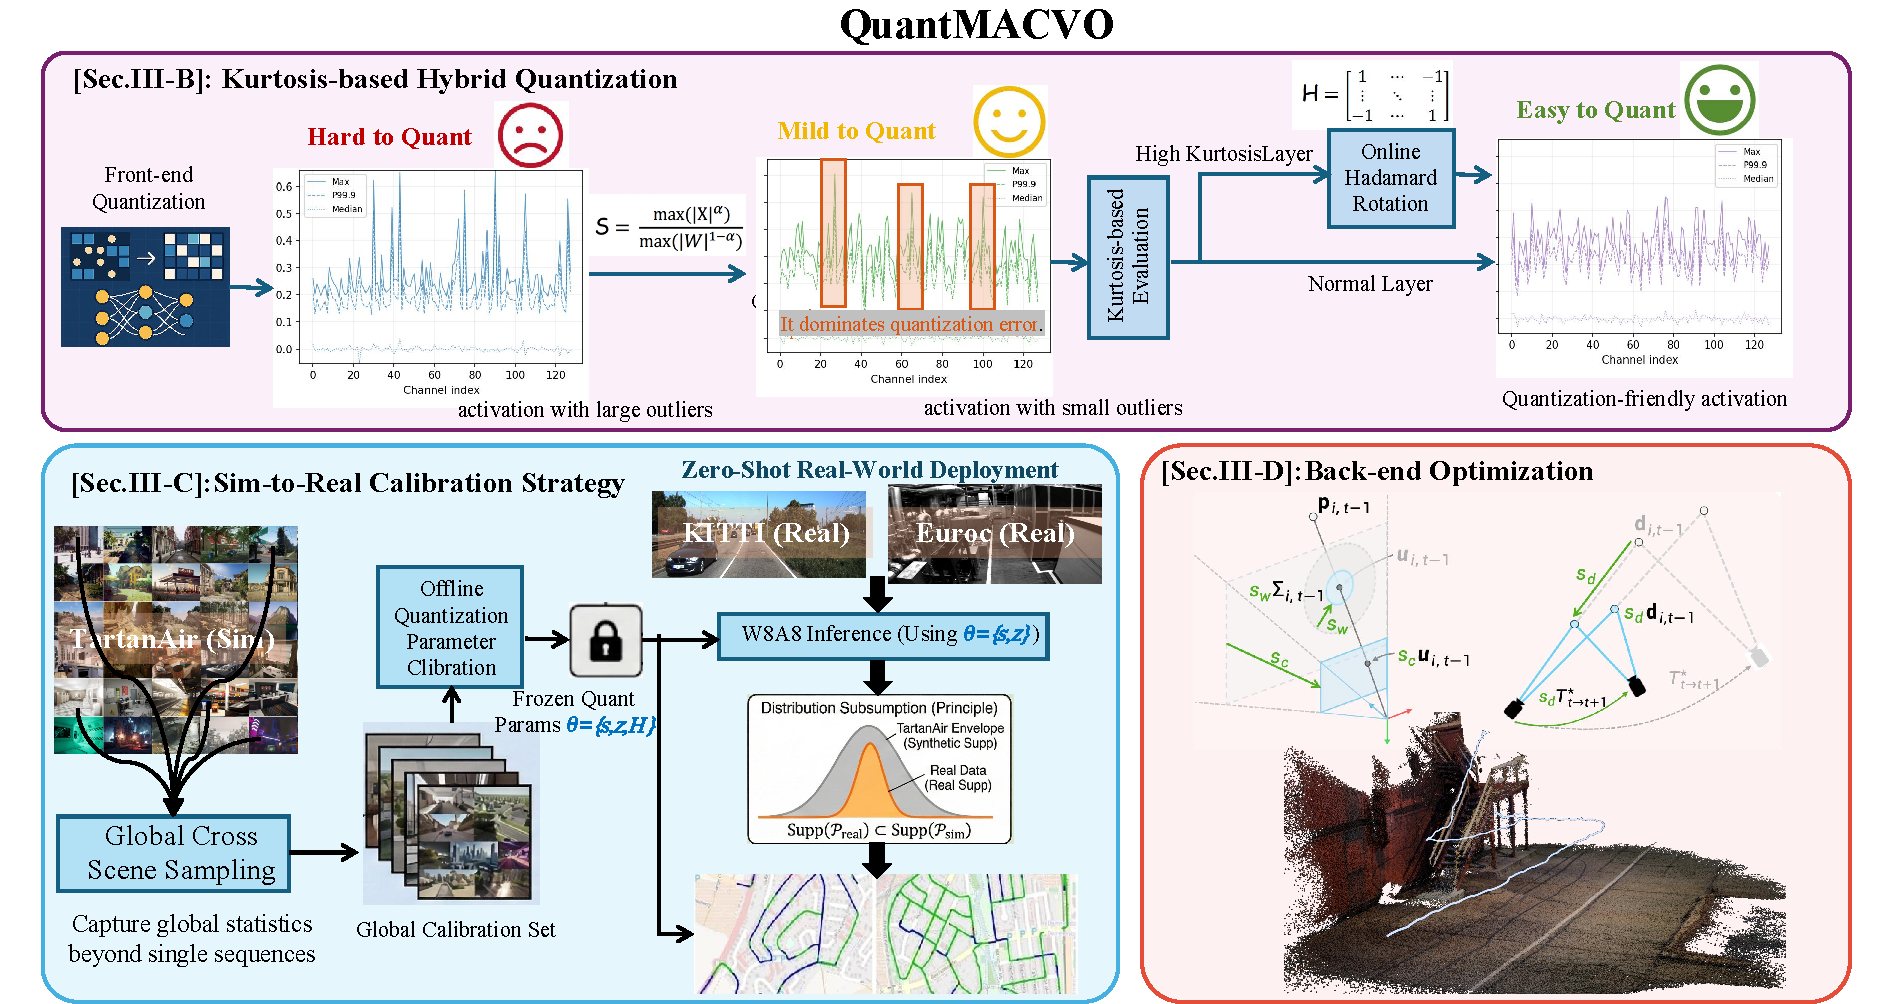
\includegraphics[width=1\textwidth]{tex/ch4_quantmacvo/figs/QuantMACVO-figures1.pdf}
  \captionsetup{font=small}
  \caption{\textbf{Overview of the QuantMAC-VO framework.} 
  \textbf{(a) Kurtosis-based Hybrid Quantization:} Layers with high kurtosis are identified via online Hadamard Rotation to suppress activation outliers. \textbf{(b) Sim-to-Real Calibration Strategy:} We construct a global calibration set from synthetic data. We derive frozen parameters ($\theta$) that envelop real-world statistics, enabling zero-shot deployment on KITTI and EuRoC.
  \textbf{(c) Back-end Optimization:} The robustly quantized features are used for precise trajectory estimation with our quantized back-end design.}
  \label{fig:framework}
\end{figure*}

\subsection{Preliminaries}
\label{sec:preliminaries}

\noindent MAC-VO~\cite{qiu2025mac} is a stereo VO system that combines a learning-based \emph{front-end} for feature matching with an optimization-based \emph{back-end}.
The front-end produces geometry cues to lift image measurements into 3D through disparity (or depth), and temporal correspondences through optical flow.
It also predicts the corresponding uncertainty for the feature matching in the keypoint selection and back-end optimization.

\noindent\textbf{Frontend (Disparity \& Flow).}
The front-end network $\mathcal{F}$ takes a rectified stereo pair $(I_{L,t}, I_{R,t})$ and a temporal left-image pair $(I_{L,t-1}, I_{L,t})$ as input.
It outputs a disparity map $\mathbf{s}_t$ for stereo triangulation and an optical flow field $\mathbf{f}_{t-1\rightarrow t}$ for temporal association, together with pixel-wise uncertainty estimates:
\begin{equation}
\label{eq:frontend_outputs}
\begin{aligned}
(\mathbf{s}_t,\, \sigma_{s,t}^2) &= \mathcal{F}(I_{L,t}, I_{R,t}), \\
(\mathbf{f}_{t-1\rightarrow t},\, \boldsymbol{\Sigma}_{\mathbf{f},t}) &= \mathcal{F}(I_{L,t-1}, I_{L,t}), \qquad
\boldsymbol{\Sigma}_{\mathbf{f},t} \triangleq
\begin{bmatrix}
\sigma_{u,t}^2 & 0\\
0 & \sigma_{v,t}^2
\end{bmatrix}.
\end{aligned}
\end{equation}

For a selected set of keypoints $\mathcal{K}$ in the left image at time $t-1$, the disparity $\mathbf{s}_{t-1}$ provides their 3D coordinates $\mathbf{p}_{k,t-1}\in\mathbb{R}^3$ via stereo triangulation.
Let $\mathbf{u}_{k,t}\in\mathbb{R}^2$ denote the 2D image coordinates of keypoint $k$ at time $t$; the flow prediction induces the correspondence
$\mathbf{u}_{k,t} = \mathbf{u}_{k,t-1} + \mathbf{f}_{k,t-1\rightarrow t}$.

\noindent\textbf{Backend (Pose Optimization).}
Given the 3D--2D correspondences $\{(\mathbf{p}_{k,t-1}, \mathbf{u}_{k,t})\}_{k\in\mathcal{K}}$, the back-end estimates the relative pose $\mathbf{T}_{t,t-1}\in SE(3)$ from frame $t\!-1$ to $t$ by minimizing a Mahalanobis-weighted reprojection error:
\begin{equation}
\label{eq:backend_pose_opt}
\mathbf{T}^\star_{t,t-1}
= \mathop{\arg\min}_{\mathbf{T}\in SE(3)}
\sum_{k\in\mathcal{K}}
\left\|\pi\bigl(\mathbf{T}\,\mathbf{p}_{k,t-1}, K\bigr) - \mathbf{u}_{k,t}\right\|^2_{\boldsymbol{\Sigma}_{\mathbf{f},k,t}},
\end{equation}
where $\pi(\,\cdot\,,K)$ is the pinhole projection with intrinsics $K$, and $\boldsymbol{\Sigma}_{\mathbf{f},k,t}$ is the  flow covariance predicted by $\mathcal F$ at keypoint $k$.

\noindent\textbf{Post-Training Quantization.} Quantization~\cite{krishnamoorthi2018quantizing, nagel2021white} converts model weights and activations from floating-point (FP) representations into low-bit integer formats, thereby reducing both computational cost and memory footprint. 
In uniform affine quantization, FP values are mapped to a fixed integer range using three key parameters: the scale factor $s$, zero-point $z$, and bit-width $b$. 
Given an FP input $\mathbf{x}$ (weights or activations), the quantization and de-quantization process can be described by \eref{eq: quant and de-quant function}, where $\lfloor \cdot \rceil$ denotes the round-to-nearest operation (RTN), and $\operatorname{clamp}(\cdot)$ restricts the result to the valid integer:
\begin{equation}
        \mathbf{x}_{\mathrm{int}} = \operatorname{clamp}\left( \left\lfloor \frac{\mathbf{x}}{s} \right\rceil + z;\, 0,\, 2^b - 1 \right), \widehat{\mathbf{x}} = s \left( \mathbf{x}_{\mathrm{int}} - z \right).
        \label{eq: quant and de-quant function}
\end{equation}
where $\mathbf{x}_{\mathrm{int}}$ represents the quantized integer value, $\hat{x}$ is the de-quantized FP value with an error that is introduced during the quantization process. 
Based on \eref{eq: quant and de-quant function}, the FP range of the quantization grid is defined as $[q_{\min},\, q_{\max}] = [-sz,\, s(2^b - 1 - z)]$. Input values $\mathbf{x}$ falling outside this range are clipped to the nearest boundary, resulting in clipping error. 
Increasing the scale factor $s$ can reduce clipping by expanding the representable range, but at the cost of increased rounding error, which is bounded within $\left[-\frac{1}{2}s,\, \frac{1}{2}s\right]$. 
To balance these two sources of error, modern quantization frameworks commonly adopt MSE-based calibration~\cite{banner2019post}, which searches for the optimal $(q_{\min}, q_{\max})$ that minimizes the Mean Squared Error (MSE) between the original tensor $\mathbf{x}$ and its de-quantized approximation $\widehat{\mathbf{x}}$.

\noindent\textbf{Rotation and Hadamard Matrices.} Recent studies~\cite{ashkboos2024quarot,yu2025mquant} have demonstrated that applying orthogonal rotations to the feature space can effectively eliminate activation outliers by redistributing feature magnitudes, yielding a more quantization-friendly distribution. In this chapter, we employ rotation matrices, defined as real orthogonal matrices $\mathbf{R}$ satisfying $\mathbf{R}\mathbf{R}^\top = \mathbf{I}$. To ensure computational efficiency during quantization, we specifically utilize the Walsh-Hadamard matrix $\mathbf{H}_d$ as the rotation operator. For a dimension $d=2^k$, $\mathbf{H}_d$ is constructed recursively using the Kronecker product $\otimes$:
\begin{equation}
    \mathbf{H}_{2^k} = \mathbf{H}_2 \otimes \mathbf{H}_{2^{k-1}}, \quad \text{with} \quad \mathbf{H}_2 = \frac{1}{\sqrt{2}}\begin{bmatrix} 1 & 1 \\ 1 & -1 \end{bmatrix}.
\end{equation}
This recursive structure enables fast matrix-vector multiplication in $\mathcal{O}(d \log_2 d)$ complexity. To further enhance the distribution flatness, we adopt the randomized Hadamard rotation $\tilde{\mathbf{H}} = \mathbf{H}_d \,\text{diag}(\mathbf{s})$, where $\mathbf{s} \in \{-1, +1\}^d$ represents a random sign vector. It is straightforward to verify that $\tilde{\mathbf{H}}$ maintains orthogonality.


\begin{figure*}[t]
  \centering
  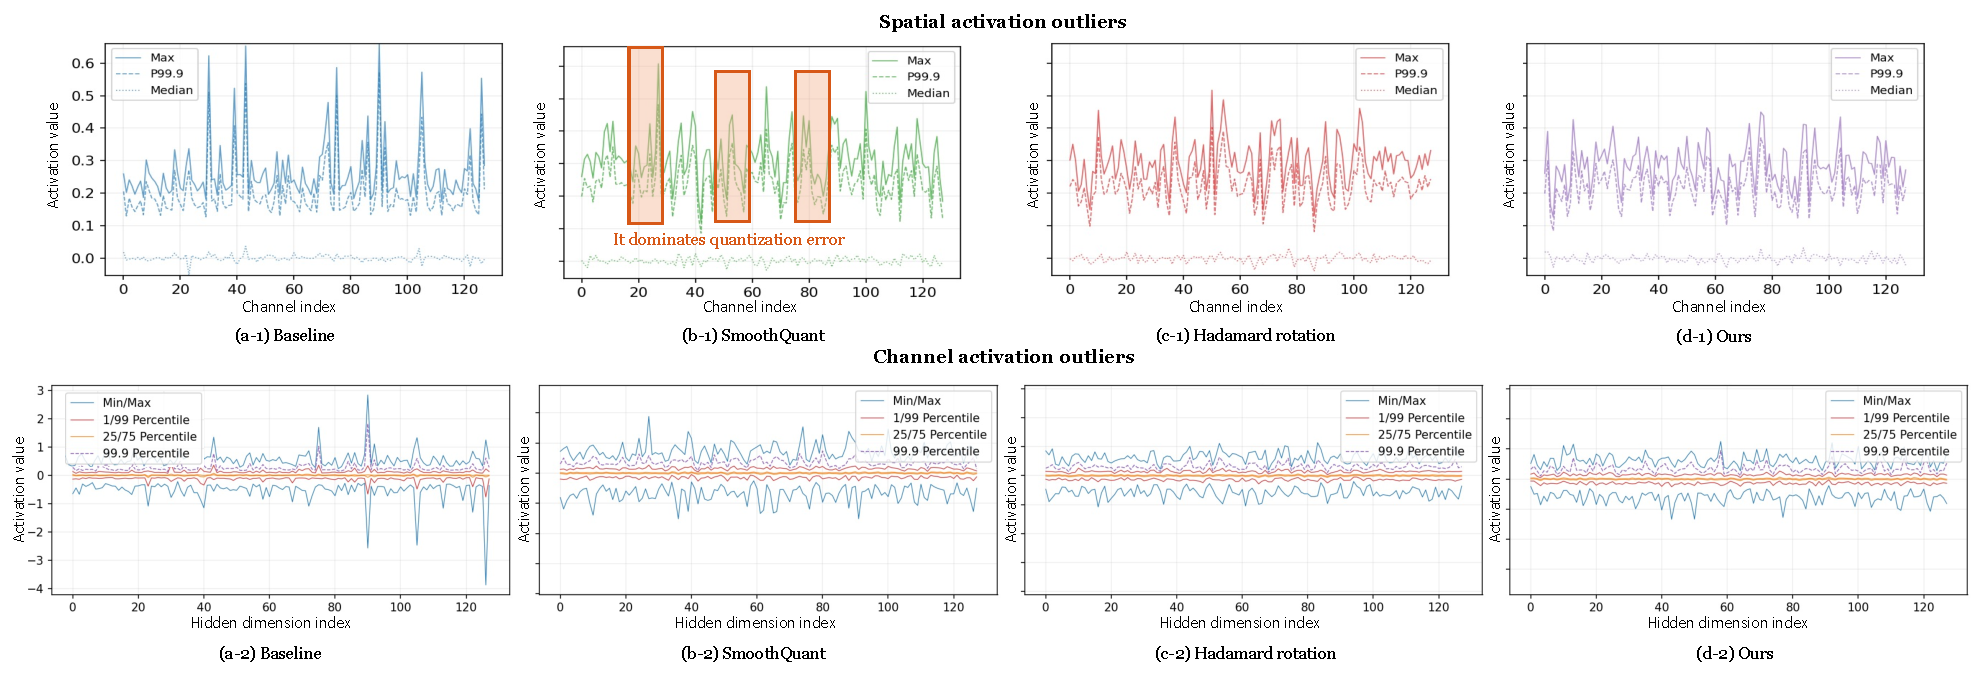
\includegraphics[width=1\textwidth]{tex/ch4_quantmacvo/figs/channel_spatial.pdf}
  \captionsetup{font=small}
  \caption{Channel and spatial outlier visualization for the conv3 activations. SmoothQuant~\cite{xiao2022smoothquant} reduces channel-wise outliers (b-2) but leaves spatially localized outliers (three hotspots in b-1). In contrast, applying a Hadamard rotation to the input activations disperses outliers across positions and channels (c-1, c-2). Our method selectively applies Hadamard rotation to outlier-dominated layers, effectively mitigating both channel- and spatial-outliers (d-1, d-2).}
  \label{fig:spatial_outlier}
\end{figure*}


\subsection{Kurtosis-based Hybrid Quantization}
\label{sec:kurtosis_hybrid}

As shown in \fref{fig:spatial_outlier}, we employ the Hadamard matrix to address both channel outliers and spatial outliers in the activations.
While effective, applying Hadamard matrices introduces additional computational overhead during quantization and inference. 
To balance quantization quality and inference latency, we propose a hybrid quantization strategy. 
Specifically, Hadamard rotation is applied only to a subset of critical layers where outliers dominate the quantization error, 
whereas the remaining layers adopt lightweight, overhead-free channel scaling~\cite{xiao2022smoothquant}.

To determine the importance of different layers, we adopt kurtosis as a selection criterion.
Kurtosis serves as a proxy metric for identifying layers that are sensitive to outliers.
Intuitively, high-kurtosis activations are dominated by a small number of extreme values, which distort the quantization grid and amplify rounding error for the remaining activations.
Compared to prior methods that rely on expensive layer-wise sensitivity profiling~\cite{zhao2024mixdq}, kurtosis-based analysis avoids redundant per-layer quantization and repeated forward passes.
In \eref{eq:kurtosis}, we compute the mean $\mu_\ell$ and variance $\sigma_\ell^2$ over the input activations of each layer $\ell$ across the analysis data, and define the layer-wise kurtosis $K_\ell$ as the standardized fourth moment from the features of each layer $X_\ell$:

\begin{equation}
  K_\ell = \frac{\mathbb{E}[(X_\ell - \mu_\ell)^4]}{\sigma_\ell^4}.
  \label{eq:kurtosis}
\end{equation}

Our kurtosis-based hybrid quantization proceeds in three steps.
(1) Kurtosis analysis: We run the full-precision model on an analysis set, compute kurtosis from the input activation distribution of each layer $l$, and normalize it to obtain a layer score $K_l$ in
\eref{eq:norm_kurtosis}.
(2) Critical layers decision: 
As shown in \fref{fig:pareto}, we choose the optimal point using the Kneedle criterion~\cite{satopaa2011kneedle}. 
The point that maximizes the difference between normalized utility and normalized cost.
We apply Hadamard rotation only up to the knee point, avoiding fixed top-$k$ choices or heuristic thresholds.
(3) PTQ calibration: After fixing the layer-wise quantization strategy, we perform our sim-to-real quantization calibration to update quantization parameters.

\begin{equation}
    \small
  \mathrm{K_{norm}}(\ell)
  = \begin{cases}
      \displaystyle\frac{K_\ell - K_{\min}}{\Delta{K}} & \text{if } \Delta{K} > 0, \\
      0 & \text{otherwise}.
    \end{cases}
    \label{eq:norm_kurtosis}
\end{equation}


\begin{figure}[t]
  \centering
  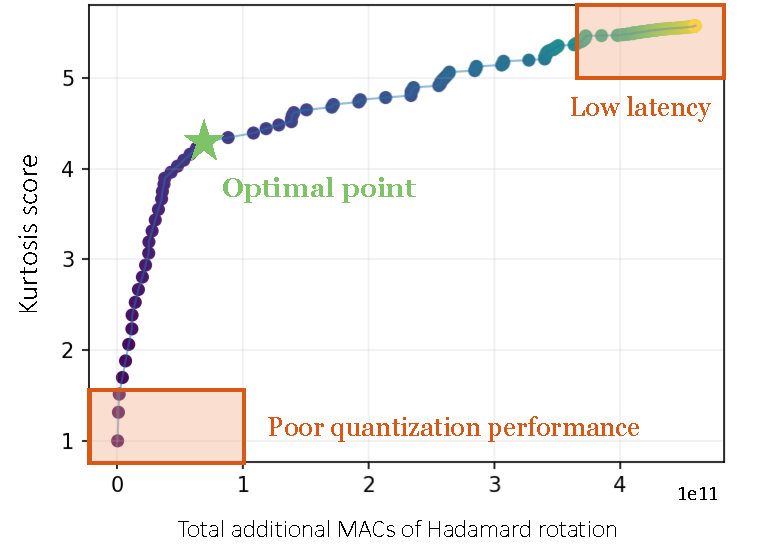
\includegraphics[width=0.5\columnwidth]{tex/ch4_quantmacvo/figs/trade_off.pdf}
  \captionsetup{font=small}
  \caption{The x-axis shows cumulative additional Multiply--Accumulate operations (MACs) of Hadamard rotation and the y-axis shows the cumulation of $K_{norm}$ up to the $i$-th layer.}
  \label{fig:pareto}
\end{figure}

\subsection{Sim-to-Real Quantization Calibration}
\label{sec:sim2real_calib}

Standard Post-Training Quantization (PTQ) algorithms~\cite{librecq,banner2019post,zhoulidar} typically rely on a small set of calibration data to determine the quantization parameters (scale factor $s$ and zero-points $z$). The prevailing wisdom suggests that this calibration set should be sampled directly from the target domain to minimize the distribution mismatch. However, in robotic applications, this requirement is often impractical. Environments are inherently dynamic and unstructured, making it infeasible to re-calibrate the model for every specific scene transition. Consequently, calibrating on a limited real-world sequence often leads to \textit{overfitting}, where narrow clipping ranges fail to accommodate unseen dynamic motions or lighting extremes, causing significant accuracy degradation or even system collapse during deployment.
To address this, we propose a {Sim-to-Real Quantization Calibration} that enables zero-shot generalization to real-world environments without requiring re-calibration on target-domain data. 

\textbf{Hypothesis of Distribution Subsumption.} Our approach is grounded in the insight that the activation statistics of robotic perception are governed by the complexity of environmental dynamics. We hypothesize that large-scale synthetic datasets, such as TartanAir \cite{tartanair}, exhibit a ``superset'' of features compared to structured real-world datasets like KITTI \cite{kitti2012} or EuRoC \cite{euroc2016}. Specifically, synthetic environments are characterized by \textit{high-entropy distributions} containing extreme optical flow magnitudes, aggressive camera rotations, and challenging texture artifacts. In contrast, real-world benchmarks often follow more predictable motion models and constrained lighting conditions. 

Therefore, we posit that the activation distribution of the target real domain $\mathcal{P}_{real}$ is statistically subsumed by the synthetic source domain $\mathcal{P}_{sim}$:
    $\text{Supp}(\mathcal{P}_{real}) \subset \text{Supp}(\mathcal{P}_{sim}),$
where $\text{Supp}(\cdot)$ denotes the support of the distribution. By calibrating on $\mathcal{P}_{sim}$, we derive a conservative \textbf{quantization envelope} that naturally encompasses the dynamic range of $\mathcal{P}_{real}$ as a subset.

\begin{figure}
  \centering
  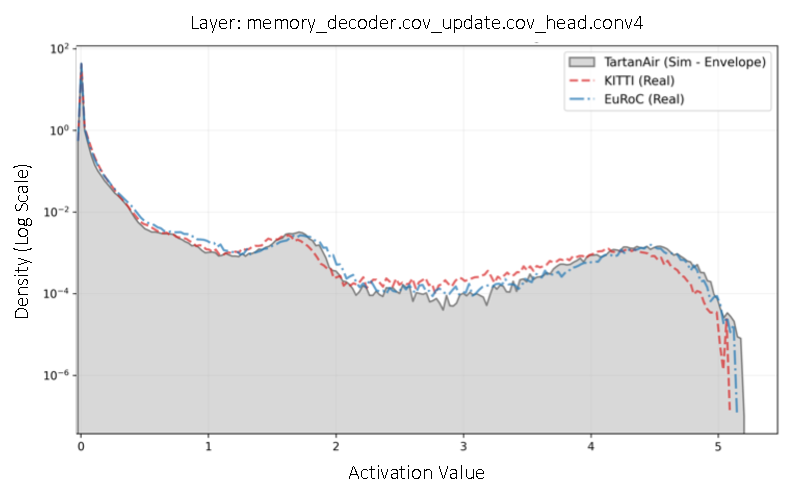
\includegraphics[width=0.5\linewidth]{tex/ch4_quantmacvo/figs/RSS_distribution_feature_1.pdf}
  \captionsetup{font=small}
  \caption{\textbf{Validation of Sim-to-Real Distribution Subsumption.} We visualize the activation density (log scale) of the middle layer in the uncertainty head. The synthetic TartanAir dataset (grey filled area) exhibits a high-entropy distribution with heavy tails, effectively forming a quantization envelope that subsumes the narrower distributions of real-world datasets (KITTI and EuRoC).}
  \label{fig:dist_analysis}
\end{figure}

This hypothesis is empirically validated in \fref{fig:dist_analysis}. The activations of the real-world datasets (KITTI and EuRoC) appear as narrow modes concentrated within a limited dynamic range. In contrast, the TartanAir distribution (grey envelope) is significantly broader, covering extreme activation values that represent challenging geometric features or lighting conditions.

\textbf{Global Cross-Scene Sampling.}
To effectively approximate the global statistics of $\mathcal{P}_{sim}$, we reject the standard practice of sampling consecutive frames from a single scene, which introduces severe temporal bias. Instead, we implement a Global Cross-Scene Sampling strategy. We construct a global calibration set $\mathcal{D}_{calib}$ by uniformly sampling frames across diverse scenes~\cite{tartanair}. This strategy ensures that the calibration set captures the maximum variance of activation outliers. 

Formally, adhering to the MSE-based calibration framework defined in \sref{sec:preliminaries}, we determine the optimal quantization range bounds $[q_{\min}, q_{\max}]$ (and subsequently $s$ and $z$) by minimizing the reconstruction error over the global synthetic set $\mathcal{D}_{calib}$:
\begin{equation}
\small
\begin{aligned}
    \small
    (q_{\min}^*, q_{\max}^*) = \operatorname*{argmin}_{q_{\min}, q_{\max}} \mathbb{E}_{\mathbf{x} \in \mathcal{D}_{calib}} \left[ \| \mathbf{x} - \widehat{\mathbf{x}}(q_{\min}, q_{\max}) \|_2^2 \right],
\end{aligned}
\end{equation}
where $\widehat{\mathbf{x}}$ is the de-quantized approximation derived via \eref{eq: quant and de-quant function}.

\textbf{Zero-Shot Generalization.}
This calibration method decouples the quantization process from the deployment environment. Calibrating on KITTI would result in a narrow clipping range (overfitting to the mode), causing severe saturation when unseen outliers occur. By calibrating on the TartanAir ``superset'', our method derives a conservative range that naturally accommodates real-world statistics. Once calibrated offline using our global synthetic set, the quantized model can be deployed ``zero-shot'' to various real-world scenes without any fine-tuning or re-calibration. As empirically validated in \sref{sec:quantmacvo_exp}, this method not only matches the accuracy of domain-specific calibration but often outperforms it by preventing the clipping of rare but critical geometric features.


\subsection{Backend Quantization}
\label{sec:backend_quant}

The backend pose estimation in \eref{eq:backend_pose_opt} is solved with a Gauss-Newton second-order optimizer. While the solver itself must remain numerically stable, the dominant implementation bottleneck is the floating-point format used for building the normal equations. Compared with FP16, BF16 offers a much wider exponent range but a coarser mantissa; its relative precision is on the order of $8\times10^{-3}$, which would bound the best-achievable translation refinement to the millimeter-centimeter scale. In contrast, FP16 provides a finer relative precision (on the order of $10^{-3}$), which is required by our back-end accuracy target. Therefore, we choose FP16 for the back-end arithmetic where possible.

However, FP16 has a limited representable dynamic range (maximum finite value on the order of $6.5\times 10^4$). In Gauss-Newton, the normal equations are formed as
\begin{equation}
\small
\label{eq:normal_equation_backend}
\mathbf{A}\,\Delta = \mathbf{b},
\quad
\mathbf{A} = \sum_k \mathbf{J}_k^\top \mathbf{W}_k \mathbf{J}_k,
\quad
\mathbf{b} = -\sum_k \mathbf{J}_k^\top \mathbf{W}_k \mathbf{r}_k,
\end{equation}
where $\mathbf{J}_k$ and $\mathbf{r}_k$ are the Jacobian and residual of the reprojection error, and $\mathbf{W}_k$ is the inverse covariance from the front-end uncertainty. Even when residuals are well-behaved, the terms in $\mathbf{A}$ can become large due to squaring and accumulation, which can overflow to $\infty/\mathrm{NaN}$ in FP16. Hence, the key challenge is to compress the numeric range of intermediate results so that building $\mathbf{A}$ and $\mathbf{b}$ remains within the FP16 range.

\begin{figure}
  \centering
  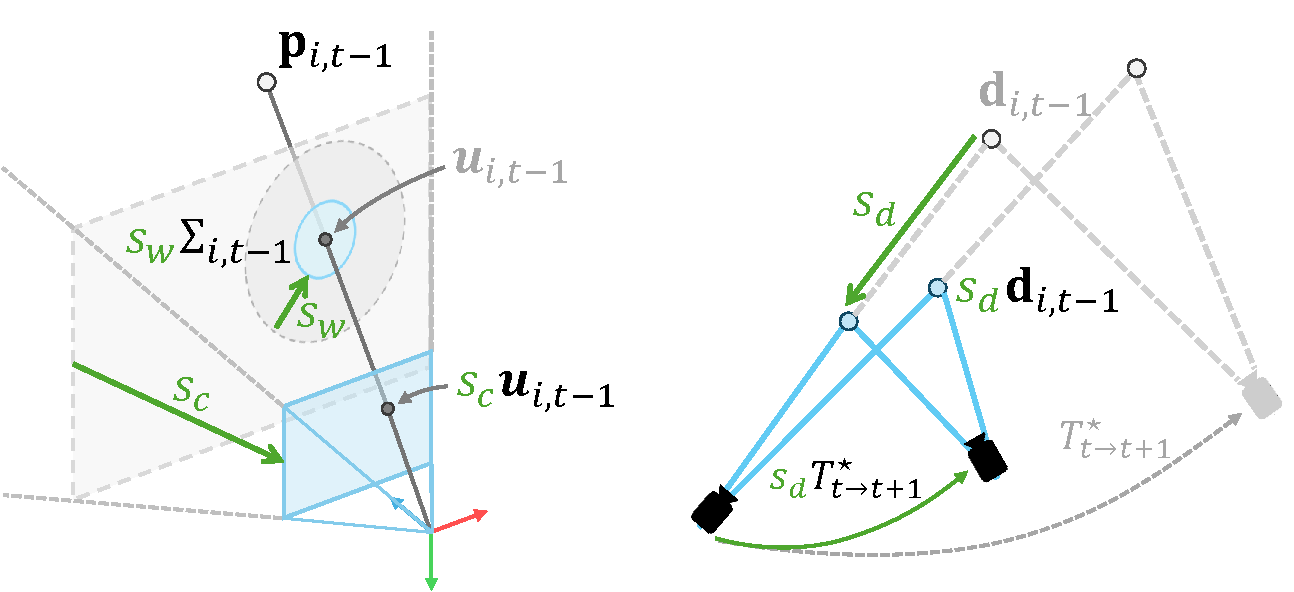
\includegraphics[width=0.6\linewidth]{tex/ch4_quantmacvo/figs/BackendScaling.pdf}
  \captionsetup{font=small}
  \caption{
  \textbf{Backend scaling factors for FP16 optimization.} 
    To prevent overflow/underflow when forming the normal equations, we rescale the backend using three factors: 
    (1) image-plane scaling $\sfactor{s_c}$ applied to pixel coordinates; 
    (2) weight scaling $\sfactor{s_w}$ applied to the inverse covariance $\mathbf{W}=\boldsymbol{\Sigma}^{-1}$; and 
    (3) 3D scaling $\sfactor{s_d}$ applied to the depths and motion.
  }
  \label{fig:backend-scale-factor}
\end{figure}

\begin{figure}
  \centering
  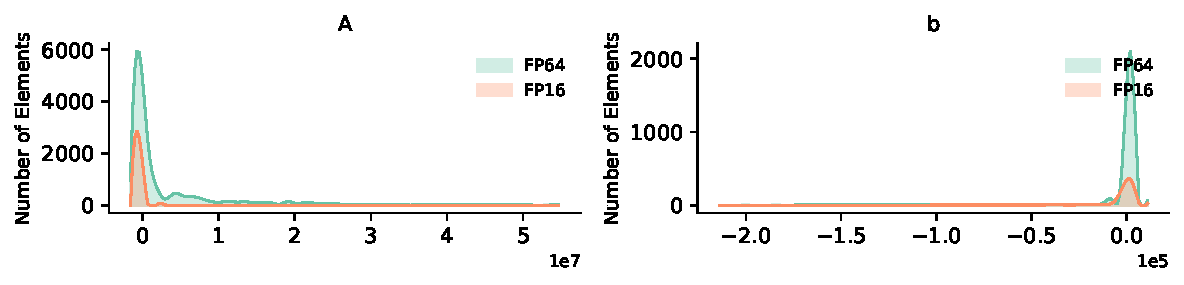
\includegraphics[width=0.6\linewidth]{tex/ch4_quantmacvo/figs/backend_distribution_naive.pdf}\\
  \vspace*{-.1cm}
  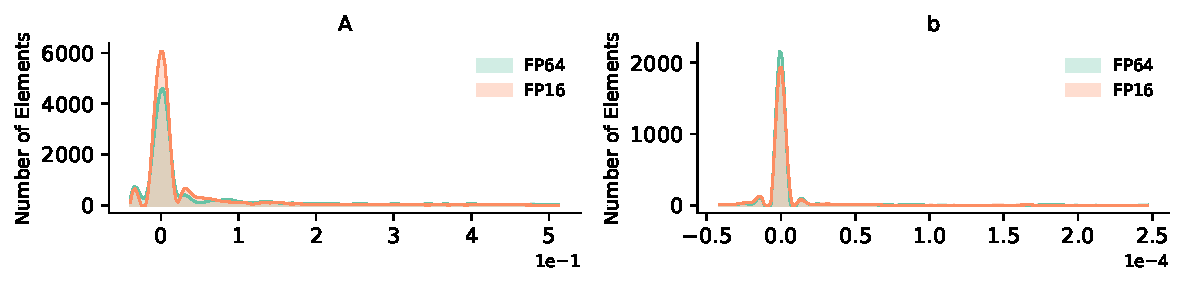
\includegraphics[width=0.6\linewidth]{tex/ch4_quantmacvo/figs/backend_distribution_scaled.pdf}
  \captionsetup{font=small}
    \caption{\textbf{Element-wise histograms of the Gauss-Newton normal equation $(\mathbf{A},\mathbf{b})$.}
    \textbf{Top:} naive FP16 suffers from dynamic-range mismatch, leading to overflow and NaN values.
    \textbf{Bottom:} our range-compression scaling brings $(\mathbf{A},\mathbf{b})$ into a stable FP16 regime, closely matching the FP64 distribution.}
  \label{fig:backend_dist_analysis}
\end{figure}

\textbf{Scale-invariant normal equations.}
Our design relies on the fact that linear systems are invariant to a non-zero scaling: $\forall s\neq 0$, $\mathbf{A}\Delta=\mathbf{b}$ and $(s\mathbf{A})\Delta=(s\mathbf{b})$ share the same solution. We exploit this invariance by applying three scale factors, as shown in \fref{fig:backend-scale-factor}, when constructing the normal equations. We provide the high-level pseudo-code of our backend in Algorithm~\ref{alg:backend_quant}.

\textbf{Weight scaling ($w$-scale).}
We scale the weight matrix by a uniform positive scalar $s_w$: $\mathbf{W}_k \leftarrow s_w\mathbf{W}_k$. This uniformly scales both $\mathbf{A}$ and $\mathbf{b}$ by $s_w$, leaving $\Delta$ unchanged, while shrinking the magnitude of the accumulated normal equations.

\textbf{Image-plane scaling ($c$-scale).}
We scale all image-plane quantities by $s_c$, including pixel observations $\mathbf{u}$, intrinsics $K$, and the robustification threshold (Huber $\delta$). Geometrically, this is equivalent to moving the image plane closer to the optical center, which shrinks the pixel coordinates and stabilizes the Jacobians. Under this scaling, both residuals and Jacobians scale as $\mathbf{r}_k\leftarrow s_j\mathbf{r}_k$ and $\mathbf{J}_k\leftarrow s_j\mathbf{J}_k$, which implies $\mathbf{A}\leftarrow s_j^2\mathbf{A}$ and $\mathbf{b}\leftarrow s_j^2\mathbf{b}$, again preserving the Gauss-Newton step.

\begin{algorithm}[t]
\small
\captionsetup{font=small}
\caption{FP16 Gauss-Newton optimization with scaling}
\label{alg:backend_quant}
\begin{algorithmic}[1]
\Require Observations $\{\mathbf{u}_{k,0}, d_{k,0}, \mathbf{u}_{k,1}^L, \mathbf{u}_{k,1}^R, \boldsymbol{\Sigma}_{k}\}_{k=1}^N$, 
\Statex \hspace{\algorithmicindent}\hspace{.8em} camera intrinsics $K$, baseline $b$, initial pose $\mathbf{T}$
\Statex \hspace{\algorithmicindent}\hspace{.8em} camera scale $\sfactor{s_c}$, 3D scale $\sfactor{s_d}$, and weight scale $\sfactor{s_w}$
\Ensure Optimized relative pose $\mathbf{T}^\star$

\State  $\mathbf{W}_k\gets \sfactor{s_w}\boldsymbol{\Sigma}_k^{-1}$
\State $\mathrm{trans}(\mathbf{T})\gets \sfactor{s_d} \cdot \mathrm{trans}(\mathbf{T})$
\For{$i=1$ to $N_{\mathrm{iter}}$}
  \State $\sfactor{s_c}\mathbf{r}_k,\sfactor{s_c}\mathbf{J}_k\gets \mathcal{E}
  (\mathbf{T};\sfactor{s_c}\mathbf{u},\sfactor{s_d}d,K,\sfactor{s_d}b)$
  \State $\sfactor{s_c}\tilde{\mathbf{r}}_k,\sfactor{s_c}\tilde{\mathbf{J}}_k\gets \mathrm{Huber}(\sfactor{s_c}\mathbf{r}_k,\sfactor{s_c}\mathbf{J}_k;\sfactor{s_c}\delta)$
  \State $\sfactor{s_ws_c^2}\mathbf{A}\leftarrow \sum_k \sfactor{s_c}\tilde{\mathbf{J}}_k^\top\sfactor{s_w}\mathbf{W}_k\sfactor{s_c}\tilde{\mathbf{J}}_k$
  \State $\sfactor{s_ws_c^2}\mathbf{b}\leftarrow -\sum_k \sfactor{s_c}\tilde{\mathbf{J}}_k^\top\sfactor{s_w}\mathbf{W}_k\sfactor{s_c}\tilde{\mathbf{r}}_k$
  \State $\Delta = \mathrm{ CholeskySolve}(\sfactor{s_ws_c^2}\mathbf{A}, \sfactor{s_ws_c^2}\mathbf{b})$ \Comment{\scriptsize FP32 Precision\normalsize}
  \scriptsize
  \State $\mathbf{T}\leftarrow \mathrm{Exp}(\Delta)\mathbf{T}$
\scriptsize
\EndFor
\scriptsize
\State $\mathrm{trans}(\mathbf{T})\gets 1/\sfactor{s_d} \cdot \mathrm{trans}(\mathbf{T})$
\State \Return $\mathbf{T}^\star\leftarrow \mathbf{T}$
\end{algorithmic}
\end{algorithm}

\textbf{3D scaling ($d$-scale).}
Finally, we scale the entire 3D geometry by a factor $s_d$ to avoid overflow in depth-dependent terms such as $(1/z)^2$. Concretely, we scale depth and baseline by $s_d$ and scale the translation component of the $SE(3)$ estimate by $s_d$ before optimization. Unlike $w$- and $j$-scales, this operation changes the physical units of translation; therefore, after the FP16 optimization converges, we explicitly restore the scale of translation by dividing $s_d$.

\textbf{Scale factor selection.}
In our implementation, the three scale factors are computed on-the-fly from simple statistics of the current frame pair.
For the image-plane scaling, we set
\begin{equation}
\label{eq:auto_s_c}
s_c = \frac{1}{\max\bigl(\mathbf{u}^L\bigr)},
\end{equation}
so that the largest observed pixel coordinate is mapped to $\mathcal{O}(1)$.
For the 3D scaling, we use depth statistics to simultaneously compress large depths and avoid overflow in $(1/z)^2$:
\begin{equation}
\small
\label{eq:auto_s_d}
s_d = \max\!\left(\frac{1}{\max(d)},\, \frac{0.01}{\min(d)}\right).
\end{equation}
The first term maps the maximum depth to roughly one, while the second enforces $s_d\min(d)\ge 0.01$ to bound $(1/z)^2$ in FP16.
Finally, after constructing per-observation weights $\mathbf{W}_k=\boldsymbol{\Sigma}_k^{-1}$, we normalize them by the maximum weight magnitude and the number of points $N$ to keep the accumulated normal equations well-scaled:
\begin{equation}
\label{eq:auto_s_w}
s_w = \frac{1}{\max_k \|\mathbf{W}_k\|\, N},\quad \mathbf{W}_k\leftarrow s_w\mathbf{W}_k.
\end{equation}

In practice, we build $\mathbf{A}$ and $\mathbf{b}$ in FP16 under the above scaling, but solve the $6\times 6$ system in FP32 via Cholesky on a symmetrized $\tfrac{1}{2}(\mathbf{A}+\mathbf{A}^\top)$ to preserve solver robustness.


\section{Experiments}
\label{sec:quantmacvo_exp}

\subsection{Implementation Details}
\label{sec:exp_impl}

\textbf{Datasets \& Baseline.}\; We follow MAC-VO~\cite{qiu2025mac} and evaluate the proposed model and baseline methods on a variety of public datasets, including synthetic dataset TartanAir v2 \cite{tartanair}, real-world data from EuRoC \cite{euroc2016}, and KITTI \cite{kitti2012}. These datasets cover a diverse range of hardware configurations, motion patterns, and environments.

\textbf{Evaluation Metrics.}\; Since the baseline~\cite{qiu2025mac} does not contain loop closure or global bundle adjustment, our evaluation follows the baseline and focuses on relative error.
We use relative translation error ($t_{\mathrm{rel}}$, $\mathrm{m/frame}$) and rotation error ($r_{\mathrm{rel}}$, $\mathrm{{}^\circ/frame}$) as:
\begin{equation}
\small
\begin{aligned}        
    t_{\mathrm{rel}} &= \frac{1}{N}\sum^N_{t=1}{\left\| \mathbf{p}_{t+1} - \mathbf{p}_{t} - R_{t}\hat{R}_{t}^\top\!\!\left(\hat{\mathbf{p}}_{t+1} - \hat{\mathbf{p}_{t}}\right)\right\|_2},\\
    r_{\mathrm{rel}} &= \frac{180}{\pi}\frac{1}{N} \sum^N_{t=1}\left\| \log\left( \hat{R}_{t,t+1}^\top  R_{t,t+1}\right)\right\|_2, 
\end{aligned}
\end{equation}
where $\mathbf{p}_t$ and $R_t$ are ground truth position and rotation, $\hat{\mathbf{p}}_t$ and $\hat{R}_t$ are the estimated position and rotation. $R_{t,t+1}= R_{t}^\top R_{t+1}$ is the rotation from frame $t$ to frame $t+1$.

\begin{table*}[t]
\centering
\captionsetup{font=scriptsize}
\caption{Performance comparison on the TartanAir v2 Hard Dataset. Average is calculated over all trajectories of TartanAir v2 Hard.}
\resizebox{\linewidth}{!}{
\begin{tabular}{lccccccccccccccccc}
\toprule
 Trajectory & W/A Bits& \multicolumn{2}{c}{{H00}} & \multicolumn{2}{c}{{H01}}  & \multicolumn{2}{c}{{H02}} & \multicolumn{2}{c}{{H03}}  & \multicolumn{2}{c}{{H04}} & \multicolumn{2}{c}{{H05}}  & \multicolumn{2}{c}{{H06}} & \multicolumn{2}{c}{Avg.} \\
\cmidrule{3-18}
   &  &$t_{\mathrm{rel}}$ & $r_{\mathrm{rel}}$ & $t_{\mathrm{rel}}$ & $r_{\mathrm{rel}}$ & $t_{\mathrm{rel}}$ & $r_{\mathrm{rel}}$ & $t_{\mathrm{rel}}$ & $r_{\mathrm{rel}}$ & $t_{\mathrm{rel}}$ & $r_{\mathrm{rel}}$ & $t_{\mathrm{rel}}$ & $r_{\mathrm{rel}}$ & $t_{\mathrm{rel}}$ & $r_{\mathrm{rel}}$ & $t_{\mathrm{rel}}$ & $r_{\mathrm{rel}}$ \\
% \rowcolor{ourgray}
\midrule
\textbf{Baseline}                     &FP32/FP32 
& 0.040 & 0.048 %H00
& 0.020 & 0.101 %H01
& 0.016 & 0.078 %H02
& 0.181 & 0.424 %H03
& 0.005 & 0.071 %H04
& 0.071 & 0.359 %H05
& 0.218 & 0.791 %H06
& 0.079 & 0.267 \\ %avg
\midrule
RTN$^\star$    &INT8/INT8              
& 1.149 & 3.839 %H00
& 0.562 & 3.529 %H01
& 0.318 & 2.225 %H02
& 0.506 & 4.578 %H03
& 0.311 & 2.436 %H04
& 0.338 & 4.717 %H05
& 0.504 & 4.185 %H06
& 0.527 & 3.644 \\ %avg
% \hspace{3mm} \stereoicon~PTQ4ViT~\cite{ptq4vit} &INT8/INT8          &-&-&-&-&-&-&-&-&-&-&-&-&-&-\\
SmoothQuant~\cite{xiao2022smoothquant}   &    INT8/INT8
& 1.102 & 3.440 %H00
& 0.371 & 2.806 %H01
& 0.243 & 1.882 %H02
& 0.382 & 3.382 %H03
& 0.202 & 1.680 %H04
& 0.292 & 3.175 %H05
& 0.337 & 3.232 %H06
& 0.419 & 2.800 \\ %avg
Quarot~\cite{ashkboos2024quarot} & INT8/INT8  
& 0.181 & 0.193 %H00
& 0.025 & 0.141 %H01
& 0.020 & 0.092 %H02
& 0.019 & 0.116 %H03
& 0.006 & 0.0880 %H04
& 0.024 & 0.386 %H05
& 0.204 & 0.825 %H06
& 0.068 & 0.263 \\ %avg
\midrule
\rowcolor{ourgray}
\textbf{Ours}                    & INT8/INT8
& 0.173 & 0.163 %H00
& 0.025 & 0.151 %H01
& 0.018 & 0.085 %H02
& 0.039 & 0.169 %H03
& 0.005 & 0.071 %H04
& 0.023 & 0.382 %H05
& 0.224 & 0.819 %H06
& 0.072 & 0.263 \\ %avg
\bottomrule
\multicolumn{17}{l}{
% \monoicon \hspace{.5mm} Monocular method.
% \quad
% \stereoicon \hspace{.5mm} Stereo method.
% \quad
$^\star$ Naive round to nearest.} \\
\end{tabular}
}
\label{tab:quantmacvo:TartanAirHard}
\end{table*}

\begin{table*}[t]
\centering
\captionsetup{font=scriptsize}
\caption{Performance comparison of different methods on the EuRoC Dataset. Average is calculated over all trajectories of EuRoC.}
\resizebox{\linewidth}{!}{
\begin{tabular}{lccccccccccccccc}
\toprule
 Trajectory & W/A Bits & \multicolumn{2}{c}{{MH01}} & \multicolumn{2}{c}{{MH03}} & \multicolumn{2}{c}{{MH05}} & \multicolumn{2}{c}{V102} & \multicolumn{2}{c}{V201} & \multicolumn{2}{c}{V203} & \multicolumn{2}{c}{Avg.} \\
\cmidrule{2-16}
   &  & $t_{\mathrm{rel}}$ & $r_{\mathrm{rel}}$ & $t_{\mathrm{rel}}$ & $r_{\mathrm{rel}}$ & $t_{\mathrm{rel}}$ & $r_{\mathrm{rel}}$ & $t_{\mathrm{rel}}$ & $r_{\mathrm{rel}}$ & $t_{\mathrm{rel}}$ & $r_{\mathrm{rel}}$ & $t_{\mathrm{rel}}$ & $r_{\mathrm{rel}}$ & $t_{\mathrm{rel}}$ & $r_{\mathrm{rel}}$ \\
\midrule
% \textbf{SLAM} \\
% \hspace{3mm} \stereoicon~ORB-SLAM 3                 & 0.0035   & 0.0450 & 0.0058   & 0.0603 & 0.0059   & 0.0526 & 0.0096   & 0.1757 & 0.0064   & 0.1615 & 0.033    & 0.9497 & 0.0092 & 0.1866 \\
% \hspace{3mm} \stereoicon~DROID-SLAM$^{\star}$          & \textbf{0.0012} & \textbf{0.0159} & 0.0034   & 0.2656 & \textbf{0.0025} & \textbf{0.0193} & \textbf{0.0026} & \textbf{0.0417} & \textbf{0.0012} & \textbf{0.0289} & \textbf{0.0034} & \textbf{0.1033} & \textbf{0.0024} & 0.0590 \\
% \hspace{3mm} \monoicon~MASt3R-SLAM$^{\star}$ & 0.0143 & 0.5493 & 0.0493 & 0.8890 & 0.0254 & 0.5808 & 0.0354 & 1.3178 & 0.0117 & 0.6818 & 0.0430 & 2.3306 & 0.0277 & 1.0472 \\
% \midrule
% \textbf{VO} \\
% \hspace{3mm} \monoicon~TartanVO$^{\star}$ &FP32/FP32  & 0.0121 & 0.0560 & 0.0302 & 0.2791 & 0.0193 & 0.0604 & 0.0251 & 0.1244 & 0.0065 & 0.0920 & 0.0303 & 0.2986 & 0.0198 & 0.1270 \\
% \hspace{3mm} \stereoicon~TartanVO &FP32/FP32                  & 0.0277 & 0.5122 & 0.0514 & 0.6635 & 0.0464 & 0.4797 & 0.0394 & 1.0420 & 0.0195 & 0.4684 & 0.0473 & 1.9657 & 0.0368 & 0.8346 \\
% \hspace{3mm} \stereoicon~iSLAM-VO  &FP32/FP32       & 0.0042 & 0.0560 & 0.0076 & 0.2789 & 0.0070 & 0.0603 & 0.0066 & 0.1241 & 0.004  & 0.0920 & 0.0151 & 0.2984 & 0.0071 & 0.1269 \\
% \hspace{3mm} \monoicon~DPVO$^{\star}$  &FP32/FP32     & 0.0015 & \underline{0.0207} & \underline{0.0028} & \underline{0.0273} & \underline{0.0028} & 0.0243 & 0.0041   & 0.0496 & \underline{0.0016} & \underline{0.0342} & \underline{0.0045} & \underline{0.1205} & \underline{0.0027} & \underline{0.0437} \\
\textbf{Baseline} &FP32/FP32        & .0014 & .0153 %MH01
& .0023 & .0187 %MH03
& .0024 & .0181 %MH05
& .0036 & .0598 %V102
& .0014 & .0339  %V201
& .0056  &.1350 %V203
& .0028 & .0468 \\%avg
\midrule
% \rowcolor{ourgray}
% \hline
RTN$^\star$    &INT8/INT8              
& .0083 & .1083 %MH01
& .0170 & .1924 %MH03
& .0204 & .1924 %MH05
& .0131 & .2240 %V102
& .0333 & .8706  %V201
& .1384  & 3.854 %V203
& .0384 & .9070 \\%avg
% \midrule
% \hspace{3mm} \stereoicon~PTQ4ViT~\cite{ptq4vit} &INT8/INT8          &-&-&-&-&-&-&-&-&-&-&-&-&-&-\\
SmoothQuant~\cite{xiao2022smoothquant}     &INT8/INT8             
& .0064 & .0937 %MH01
& .0107 & .1161 %MH03
& .0123 & .1037 %MH05
& .0104 & .1962 %V102
& .0067 & .1499  %V201
& .0358  & 1.033 %V203
& .0137 & .4226 \\%avg
Quarot~\cite{ashkboos2024quarot}      &INT8/INT8            
& .0015 & .0195 %MH01
& .0026 & .0251 %MH03
& .0031 & .0248 %MH05
& .0046 & .0848 %V102
& .0022 & .0460  %V201
& .0078  & .1646 %V203
& .0036 & .0608 \\%avg
\midrule
\rowcolor{ourgray} \textbf{Ours}  &INT8/INT8                
& .0013 & .0167 %MH01
& .0024 & .0213 %MH03
& .0026 & .0207 %MH05
& .0036 & .0572 %V102
& .0016 & .0368  %V201
& .0059  & .1412 %V203
& .0029 & .0490 \\%avg

\bottomrule
\multicolumn{12}{l}{
% $^\ddagger$ Average over all trajectories of EuRoC.
\quad
% \monoicon~\hspace{.5mm} Monocular method.
% \quad
% \stereoicon~\hspace{.5mm} Stereo method.
% \quad
$^\star$ Naive round to nearest.} \\
\end{tabular}
}
\label{tab:quantmacvo:EuRoC}
\end{table*}
\begin{table*}[t]
\centering
\captionsetup{font=scriptsize}
\caption{Performance comparison of different methods on the KITTI Dataset. Average is calculated over all trajectories of KITTI Odometry.}
\resizebox{\linewidth}{!}{
\begin{tabular}{lccccccccccccccc}
\toprule
 Trajectory &W/A Bits & \multicolumn{2}{c}{{00}} & \multicolumn{2}{c}{{02}} & \multicolumn{2}{c}{{04}} & \multicolumn{2}{c}{06} & \multicolumn{2}{c}{08} & \multicolumn{2}{c}{10} & \multicolumn{2}{c}{Avg.} \\
\cmidrule{3-16}
   &  &$t_{\mathrm{rel}}$ & $r_{\mathrm{rel}}$ & $t_{\mathrm{rel}}$ & $r_{\mathrm{rel}}$ & $t_{\mathrm{rel}}$ & $r_{\mathrm{rel}}$ & $t_{\mathrm{rel}}$ & $r_{\mathrm{rel}}$ & $t_{\mathrm{rel}}$ & $r_{\mathrm{rel}}$ & $t_{\mathrm{rel}}$ & $r_{\mathrm{rel}}$ & $t_{\mathrm{rel}}$ & $r_{\mathrm{rel}}$ \\
% \midrule
% \textbf{SLAM} \\
% \hspace{3mm} \stereoicon~ORB-SLAM 3         & 0.0252   & 0.0586 & 0.0438   & 0.0529 & 0.0274   & 0.0322 & 0.0228   & 0.0338 & \underline{0.0271} & 0.0455 & \textbf{0.0166} & \underline{0.0515} & \textbf{0.0258} & \underline{0.0434} \\
% \hspace{3mm} \stereoicon~DROID-SLAM$^\star$  & \underline{0.0198} & \underline{0.0538} & \underline{0.0250} & \underline{0.0445} & \underline{0.0255} & \underline{0.0296} & \underline{0.0199} & \underline{0.0296} & 0.0275   & \underline{0.0381} & 0.0309  & 0.0715 & 0.0900 & 0.0448 \\
% \hspace{3mm} \monoicon~MASt3R-SLAM$^{\star}$ & 0.8988 & 0.7154 & 1.0104 & 0.5959 & 1.2266 & 0.1124 & 1.2599 & 0.1289 & 0.7760 & 0.6075 & 0.6889 & 0.4709 & 0.9538 & 0.4202 \\
\midrule
\textbf{Baseline}                           & FP32/FP32
& .0176 & .0510 
& .0196 & .0400
& .0146 & .0243
& .0127 & .0279
& .0223 & .0338 
& .0115 & .0391
& .0164 & .0360 \\
\midrule
RTN$^\star$    &INT8/INT8              
& .2664 & .3718 %00
& .4393 & .5070 %02
& .9022 & .2346 %04
& .6867 & .1980 %06
& .2618 & .3205  %08
& .2654  & .3432 %10
& .4703 & .3292 \\%avg
% \hspace{3mm} \stereoicon~PTQ4ViT~\cite{ptq4vit} &INT8/INT8          &-&-&-&-&-&-&-&-&-&-&-&-&-&-\\
SmoothQuant~\cite{xiao2022smoothquant}   & INT8/INT8 
& .1747 & .2455 %00
& .1885 & .1966 %02
& .8191 & .1460 %04
& .4060 & .2314 %06
& .1883 & .2139  %08
& .2973  & .2461 %10
& .3456 & .2132 \\%avg
Quarot~\cite{ashkboos2024quarot}   & INT8/INT8 
& .0176 & .0523 %00
& .0196 & .0410 %02
& .0140 & .0262 %04
& .0122 & .0288 %06
& .0224 & .0352  %08
& .0119  & .0404 %10
& .0163 & .0373 \\%avg
\midrule
\rowcolor{ourgray}
\textbf{Ours}                           & INT8/INT8
& .0174 & .0518 %00
& .0195 & .0405 %02
& .0139 & .0254 %04
& .0121 & .0297 %06
& .0223 & .0345  %08
& .0117  & .0396 %10
& .0161 & .0369 \\%avg
\bottomrule
\multicolumn{15}{l}{
% $^\ddagger$ Average over all trajectories (from 00 to 10) of KITTI Odom.
% \quad
% \monoicon \hspace{.5mm} Monocular method.
% \quad
% \stereoicon \hspace{.5mm} Stereo method.
% \quad
$^\star$ Naive round to nearest.} \\
\end{tabular}
}
\label{tab:quantmacvo:KITTI}
\end{table*}


\subsection{Quantization Accuracy Comparison}
\label{sec:quant_accuracy}

\textbf{TartanAir v2 Dataset.}\;\;
TartanAir v2~\cite{tartanair} presents significant challenges for visual odometry due to its rigorous motion and extreme illumination changes. We evaluate our quantization method on the challenging TartanAir v2 Hard dataset, as shown in \tref{tab:quantmacvo:TartanAirHard}. Standard methods suffer severe degradation under these extreme conditions; naive RTN and SmoothQuant~\cite{xiao2022smoothquant} yield high translation and rotation errors, respectively, failing to handle the dynamic activation range. In contrast, our method achieves state-of-the-art performance, outperforming SmoothQuant and matching the advanced rotation-based method Quarot~\cite{ashkboos2024quarot}. Crucially, our W8A8 model achieves near-lossless accuracy compared to the FP32 baseline, confirming that our approach preserves geometric fidelity for efficient inference.


\textbf{EuRoC Dataset.}\;\;
To validate the real-world generalization capability of our method, we evaluate on the EuRoC MAV dataset~\cite{euroc2016}, which features aggressive flight dynamics. As shown in \tref{tab:quantmacvo:EuRoC}, standard post-training quantization methods (naive RTN) struggle to maintain trajectory precision; and SmoothQuant~\cite{xiao2022smoothquant} yields large translation and rotation errors, representing a significant degradation compared to the FP baseline. In contrast, our method achieves an average $t_{\mathrm{rel}}$ of 0.003, significantly outperforming SmoothQuant and even surpassing the rotation-based Quarot~\cite{ashkboos2024quarot} (0.004). Notably, our W8A8 model delivers near-lossless accuracy virtually identical to the FP32 baseline, empirically confirming that our Sim-to-Real calibration strategy robustly covers real-world statistics for zero-shot deployment.


\textbf{KITTI Dataset.}\;
To further validate our robustness and consistency in outdoor settings, we evaluate our method on the KITTI Odometry dataset~\cite{kitti2012}, a standard benchmark for outdoor autonomous driving characterized by large-scale urban scenes and high-speed motion. As presented in \tref{tab:quantmacvo:KITTI}, naive RTN and SmoothQuant~\cite{xiao2022smoothquant} exhibit significant performance drops in this complex outdoor environment, failing to maintain reliable localization. In contrast, our method demonstrates exceptional robustness, consistently achieving state-of-the-art accuracy across all trajectories. Most notably, our W8A8 model delivers near-lossless performance virtually indistinguishable from the FP32 baseline, proving that our Sim-to-Real calibration strategy effectively captures the activation statistics required for zero-shot deployment in autonomous driving applications.

 
\subsection{Scaling Laws for Sim-to-Real Calibration} 
\label{sec:scaling_law}

\begin{table*}[t]
    \scriptsize
    \centering
    \captionsetup{font=scriptsize}
    \caption{\textbf{Scaling Laws for Sim2Real Quantization Calibration.} We evaluate the quantization performance on relative translation error ($t_{\mathrm{rel}}$, $\mathrm{m/frame}$) and rotation error ($r_{\mathrm{rel}}$, $\mathrm{{}^\circ/frame}$) across synthetic and real-world datasets as we increase the size and diversity of the synthetic calibration set ($\mathcal{D}_{calib}$). The calibration frames are uniformly sampled from increasing numbers of TartanAir sequences.}
    \label{tab:quantmacvo:scaling_law}
    \resizebox{\linewidth}{!}{
    \begin{tabular}{l|c|c|cc|cc|cc|cc}
        \toprule
        \multirow{2}{*}{\textbf{Calibration Source}} & \textbf{Calib. Size} &\multirow{2}{*}{\textbf{W/A Bits}} & \multicolumn{2}{c|}{\textbf{TartanAir (Sim)}} & \multicolumn{2}{c|}{\textbf{EuRoC (Real)}} & \multicolumn{2}{c|}{\textbf{KITTI (Real)}} & \multicolumn{2}{c}{\textbf{Avg.}}\\
        & (\# Frames) & & $r_{\mathrm{rel}}$ & $t_{\mathrm{rel}}$ & $r_{\mathrm{rel}}$ & $t_{\mathrm{rel}}$ & $r_{\mathrm{rel}}$ & $t_{\mathrm{rel}}$ & $r_{\mathrm{rel}}$ & $t_{\mathrm{rel}}$ \\
        \midrule
        \multicolumn{2}{l|}{Baseline} &FP32 / FP32 & 0.079 & 0.267 & .0028 & .0468 & .0164 & .0360 & .0351 & .1246 \\
        \midrule
        Target Domain Calib.$^\star$ & 256 &INT8 / INT8 & .0743 & .2680 & .0028 & .0469 & .0163 & .0361 & .0290 & .1250 \\
        \midrule
        \multirow{6}{*}{\textbf{Ours (Sim-Calib)}} 
        & 16  &INT8 / INT8 & .0855 & .3326 & .0029 & .0488 & .0161 & .0370 & .0338 & .1494 \\
        & 32  &INT8 / INT8 & .0811 & .2938 & .0029 & .0487 & .0162 &.0368  & .0359 & .1352 \\
        & 64   &INT8 / INT8 & .0755 & .2838 & .0029 & .0481 & .0162 & .0364 & .0356 & .1315 \\
        & 128  &INT8 / INT8 & .0750 & .2813 & .0028 & .0478 & .0161 & .0365 & .0294 & .1309 \\
        & 256 &INT8 / INT8 & .0748 & .2780 & .0028 & .0475 & .0161 & .0363 & .0292 & .1292 \\
        & 512 &INT8 / INT8 & .0748 & .2778 & .0028 & .0476 & .0162 & .0362 & .0291 & .1293\\
        \bottomrule
        \multicolumn{3}{l}{
\quad
$^\star$ Standard PTQ calibrated on the test domain itself.} \\
    \end{tabular}
    }
    \label{tab:quantmacvo:calib}
\end{table*}
\begin{table*}[hbtp]
    \scriptsize
    \centering
    \captionsetup{font=scriptsize}
    \caption{We progressively validate the effectiveness of each proposed component, including Hybrid Quantization (Hybrid Quant), Sim-to-Real Calibration (Sim2Real Calib), and Backend Quantization (Backend Quant). The results demonstrate that each module contributes significantly to recovering the performance of the quantized model.}
    \label{tab:quantmacvo:ablation}
    \resizebox{0.9\linewidth}{!}{
    \begin{tabular}{l|c|cc|cc|cc|cc}
        \toprule
        \multirow{2}{*}{\textbf{Setting}} &\multirow{2}{*}{\textbf{W/A Bits}} & \multicolumn{2}{c|}{\textbf{TartanAir (Sim)}} & \multicolumn{2}{c|}{\textbf{EuRoC (Real)}} & \multicolumn{2}{c|}{\textbf{KITTI (Real)}} & \multicolumn{2}{c}{\textbf{Avg.}}\\
       & & $r_{\mathrm{rel}}$ & $t_{\mathrm{rel}}$ & $r_{\mathrm{rel}}$ & $t_{\mathrm{rel}}$ & $r_{\mathrm{rel}}$ & $t_{\mathrm{rel}}$ & $r_{\mathrm{rel}}$ & $t_{\mathrm{rel}}$ \\
        \midrule
        FP Model &FP32 / FP32 & .0790 & 0.2670 & .0028 & .0468 & .0164 & .0360 & .0351 & .1246 \\
        \midrule
         RTN  &INT8 / INT8 & .5270 & 3.644 & .0384 & .9070 & .4703 & .3292 & .4639 & 1.733 \\
         + Hybrid Quant  &INT8 / INT8 & .0770 & .2840 & .0035 & .0550 & .0182 & .0373 & .0352 & .1338 \\
         + Sim2Real Calib  &INT8 / INT8 & .0720 & .2630 & .0029 & .0490 & .0161 & .0369 & .0325 & .1240 \\
         \rowcolor{ourgray} + Backend Quant & INT8 / INT8 & .0748 & .2780 & .0028 & .0475 & .0161 & .0363 & .0335 & .1288 \\
        \bottomrule
    \end{tabular}
    }
\end{table*}

To validate our hypothesis that a sufficiently diverse synthetic calibration set can encompass real-world statistics, we investigate the \textbf{scaling laws} of our calibration method. We vary the size of the global calibration set $\mathcal{D}_{calib}$ by uniformly sampling frames from an increasing number of synthetic TartanAir environments (ranging from 16 to 512 frames). We then evaluate the quantized model's zero-shot performance across three distinct domains: the unseen TartanAir test split, KITTI (outdoor driving), and EuRoC (indoor MAV). The quantitative results are summarized in \tref{tab:quantmacvo:scaling_law}.

\textbf{Sim-to-Real Correlation.}
We observe a strong correlation between the diversity of synthetic calibration data and cross-domain generalization. As the calibration size increases from 16 to 256 frames, the relative translation error ($t_{\mathrm{rel}}$) decreases monotonically. Crucially, the performance gains on the synthetic validation set (TartanAir) translate directly to the real-world benchmarks. This empirically confirms our \textit{Distribution Subsumption} hypothesis: by capturing the long-tail distribution of the synthetic ``superset'', we progressively construct a robust quantization envelope that inherently covers the subsets of real-world statistics.

\textbf{Saturation and Efficiency.} The performance improvement follows a logarithmic trend, showing rapid gains initially and saturating around 256 frames. Extending the calibration size to 512 frames yields negligible marginal gains, indicating that the quantization parameters have converged to an optimal ``envelope'' that accommodates potential outliers.



% \definecolor{ourgray}{gray}{0.92}

% \begin{table*}[htbp]
% \centering
% \captionsetup{font=small}
% \caption{Latency comparison of different methods on various image resolutions for front-end/back-end (ms) and overall throughput (fps) in NVIDIA Jetson Thor. SmoothQuant~\cite{xiao2022smoothquant} is theoretically equal latency with RTN.}
% \resizebox{\linewidth}{!}{
% \setlength{\tabcolsep}{3.5pt}
% \renewcommand{\arraystretch}{1.15}

% \begin{tabular}{l
% *{5}{c}      % Baseline (5)
% *{5}{c}      % RTN / SmoothQuant (5)
% *{5}{c}      % RTN / SmoothQuant (5) -- second block
% *{4}{c}      % Ours (Front 2 + Back 2)
% >{\columncolor{ourgray}}c  % Ours Overall (fps) ONLY
% }
% \toprule

%  & \multicolumn{5}{c}{\textbf{Baseline}}
%  & \multicolumn{5}{c}{\textbf{RTN / SmoothQuant}$^\ast$}
%  & \multicolumn{5}{c}{\textbf{Quarot}$^\ast$}
%  & \multicolumn{5}{c}{\textbf{Ours}} \\
% \cmidrule(lr){2-6}\cmidrule(lr){7-11}\cmidrule(lr){12-16}\cmidrule(lr){17-21}

% Resolution
% & \multicolumn{2}{c}{Front-end} & \multicolumn{2}{c}{Back-end} & Overall
% & \multicolumn{2}{c}{Front-end} & \multicolumn{2}{c}{Back-end} & Overall
% & \multicolumn{2}{c}{Front-end} & \multicolumn{2}{c}{Back-end} & Overall
% & \multicolumn{2}{c}{Front-end} & \multicolumn{2}{c}{Back-end} & Overall \\
% \cmidrule(lr){2-3}\cmidrule(lr){4-5}\cmidrule(lr){6-6}
% \cmidrule(lr){7-8}\cmidrule(lr){9-10}\cmidrule(lr){11-11}
% \cmidrule(lr){12-13}\cmidrule(lr){14-15}\cmidrule(lr){16-16}
% \cmidrule(lr){17-18}\cmidrule(lr){19-20}\cmidrule(lr){21-21}

%  & Q$_{50}$ & Q$_{95}$ & Q$_{50}$ & Q$_{95}$ & fps
%  & Q$_{50}$ & Q$_{95}$ & Q$_{50}$ & Q$_{95}$ & fps
%  & Q$_{50}$ & Q$_{95}$ & Q$_{50}$ & Q$_{95}$ & fps
%  & Q$_{50}$ & Q$_{95}$ & Q$_{50}$ & Q$_{95}$ & fps \\
% \midrule

% 640$\times$640
% & 546.8 & 551.3 & 20.5 & 30.3 & 1.66
% & 197.5 & 201.4 & 19.2 & 31.3 & 3.90
% & 726.4 & 808.5 & 21.8 & 32.7 & 1.27
% & 243.0 & 246.2 & 16.7 & \textbf{17.8} & \textbf{3.35} \\

% 480$\times$640
% & 376.2 & 399.8 & 22.5 & 33.0 & 2.30
% & 140.0 & 143.6 & 22.2 & 32.2 & 5.08
% & 501.0 & 538.9 & 22.2 & 32.4 & 1.79
% & 180.4 & 183.7 & 16.6 & \textbf{17.9} & \textbf{4.33} \\

% 320$\times$320
% & 120.8 & 123.4 & 18.1 & 28.7 & 5.53
% & 47.6 & 49.5 & 18.8 & 29.9 & 9.37
% & 126.3 & 129.0 & 19.1 & 30.7 & 5.40
% & 57.5 & 59.6 & 16.7 & \textbf{18.5} & \textbf{8.76} \\

% 224$\times$224
% & 62.3 & 63.8 & 16.4 & 25.1 & 8.30
% & 28.3 & 30.3 & 16.7 & 25.4 & 11.72
% & 60.3 & 62.5 & 16.5 & 25.8 & 8.48
% & 33.5 & 35.5 & 16.3 & \textbf{25.8} & \textbf{10.91} \\

% \bottomrule
% \end{tabular}
% }
% \vspace{-4pt}
% \label{tab:latency_quantiles_by_resolution}
% \end{table*}


\definecolor{ourgray}{gray}{0.92}

% \begin{table}[htbp]
% \centering
% \captionsetup{font=small}
% \caption{Latency comparison of different methods on various image resolutions for overall throughput (fps) in NVIDIA Jetson Thor. SmoothQuant~\cite{xiao2022smoothquant} is theoretically equal latency with RTN.}
% \resizebox{\linewidth}{!}{
% \setlength{\tabcolsep}{6pt}
% \renewcommand{\arraystretch}{1.15}

% \begin{tabular}{l
% c  % Baseline fps
% c  % RTN / SmoothQuant fps
% c  % Quarot fps
% >{\columncolor{ourgray}}c  % Ours fps shaded
% }
% \toprule
% Resolution & \textbf{Baseline} & \textbf{RTN / SmoothQuant~\cite{xiao2022smoothquant}} & \textbf{Quarot}$^\ast$ & \textbf{Ours} \\
% \midrule
% 640$\times$640 & 1.66 & 3.90 & 1.27 & \textbf{3.35} \\
% 480$\times$640 & 2.30 & 5.08 & 1.79 & \textbf{4.33} \\
% 320$\times$320 & 5.53 & 9.37 & 5.40 & \textbf{8.76} \\
% 224$\times$224 & 8.30 & 11.72 & 8.48 & \textbf{10.91} \\
% \bottomrule
% \end{tabular}
% }
% \vspace{-4pt}
% \label{tab:fps_only_by_resolution}
% \end{table}

% \definecolor{ourgray}{gray}{0.92}

% \begin{table}[htbp]
% \centering
% \captionsetup{font=small}
% \caption{Latency comparison of different methods on various image resolutions for overall throughput (fps) in NVIDIA Jetson Thor. SmoothQuant~\cite{xiao2022smoothquant} is theoretically equal latency with RTN. All methods are evaluated under W8A8.}
% \resizebox{\linewidth}{!}{
% \setlength{\tabcolsep}{6pt}
% \renewcommand{\arraystretch}{1.15}

% \begin{tabular}{l
% c  % Baseline fps
% c  % RTN fps
% c  % SmoothQuant fps
% c  % Quarot fps
% >{\columncolor{ourgray}}c  % Ours fps shaded
% }
% \toprule
% Resolution & \textbf{Baseline} & \textbf{RTN} & \textbf{SmoothQuant~\cite{xiao2022smoothquant}} & \textbf{Quarot~\cite{ashkboos2024quarot}} & \textbf{Ours} \\
% \midrule
% 640$\times$640 & 1.16 & 3.90 & 3.90 & 1.27 & \textbf{3.35} \\
% 480$\times$640 & 1.67 & 5.08 & 5.08 & 1.79 & \textbf{4.33} \\
% 320$\times$320 & 4.78 & 9.37 & 9.37 & 5.40 & \textbf{8.76} \\
% 224$\times$224 & 7.67 & 11.72 & 11.72 & 8.48 & \textbf{10.91} \\
% \bottomrule
% \end{tabular}
% }
% \vspace{-4pt}
% \label{tab:fps_only_by_resolution}
% \end{table}


\definecolor{ourgray}{gray}{0.92}
\newcommand{\up}[1]{{\scriptsize($\uparrow\!\!#1\!\times$)}}
\newcommand{\down}[1]{{\scriptsize($\downarrow\!\!#1\times$)}}

\begin{table}[htbp]
\centering
\captionsetup{font=scriptsize}
\caption{End-to-end latency comparison on NVIDIA Jetson Thor across input image resolutions under W8A8, reported as throughput (fps).
SmoothQuant~\cite{xiao2022smoothquant} is theoretically equal latency with RTN.}
\resizebox{0.7\columnwidth}{!}{
\begin{tabular}{l c c c >{\columncolor{ourgray}}c}
\toprule
\textbf{Resolution} & \textbf{Baseline} & \textbf{RTN/SmoothQuant~\cite{xiao2022smoothquant}} & \textbf{Quarot~\cite{ashkboos2024quarot}} & \textbf{Ours} \\
\midrule
640$\times$640 & 1.16
& 3.90 \up{3.36}
& 1.27 \up{1.09}
& \textbf{3.35} \up{2.89} \\

480$\times$640 & 1.67
& 5.08 \up{3.04}
& 1.79 \up{1.07}
& \textbf{4.33} \up{2.59} \\

320$\times$320 & 4.78
& 9.37 \up{1.96}
& 5.40 \up{1.13}
& \textbf{8.76} \up{1.83} \\

224$\times$224 & 7.67
& 11.72 \up{1.53}
& 8.48 \up{1.11}
& \textbf{10.91} \up{1.42} \\
\bottomrule
\end{tabular}
}
\label{tab:quantmacvo:fps}
\end{table}



\subsection{Latency Evaluation}
\label{sec:latency_eval}

We evaluate runtime efficiency by deploying our model on NVIDIA Jetson Thor and measuring end-to-end latency, comparing against the FP32 MAC-VO baseline and quantized baselines including RTN, SmoothQuant~\cite{xiao2022smoothquant}, and QuaRot~\cite{ashkboos2024quarot}.
We report throughput in fps (frames per second).
All methods are evaluated under W8A8.
Each quantized model is exported to ONNX~\cite{onnx} and compiled into a TensorRT~\cite{nvidia_tensorrt} engine for deployment. The FP32 baseline is measured using the original MAC-VO~\cite{qiu2025mac} implementation. We fix the network depth of the front-end to 12 and evaluate latency on different image resolutions from 224$\times$224 to 640$\times$640.

As shown in \tref{tab:quantmacvo:fps}, applying Hadamard rotation to all quantized layers (QuaRot~\cite{ashkboos2024quarot}) provides only a marginal speedup (avg. 1.1$\times$ FPS). This indicates that the rotation computations incur noticeable latency overhead. In contrast, our method achieves up to 2.9$\times$ speedup over the entire baseline, despite the added rotation operations. 
RTN and SmoothQuant~\cite{xiao2022smoothquant} introduce no additional inference-time operators. However, they show higher FPS across all resolutions but suffer from accuracy degradation as discussed in \sref{sec:quant_accuracy}.


\subsection{Ablation Study}
\label{sec:ablation_quantmacvo}

To verify the effect of each component in our framework, we conduct a comprehensive ablation study as shown in \tref{tab:quantmacvo:ablation}. Directly applying standard Round-to-Nearest (RTN) quantization leads to catastrophic degradation, increasing the average relative translation error, rendering the system unusable. After introducing our Hybrid Quant strategy, it significantly mitigates quantization noise, recovering the majority of the accuracy. Furthermore, by incorporating our Sim-to-Real Calibration method with global synthetic sampling, the model achieves better generalization on real-world datasets. Finally, with the inclusion of our backend quantization, the fully integrated system achieves performance comparable to the FP32 baseline, ensuring robust deployment across diverse environments.


\section{Sim-to-Real Calibration Performance Curve}
\label{sec:sim2real_curve}

\begin{figure}[h]
  \centering
  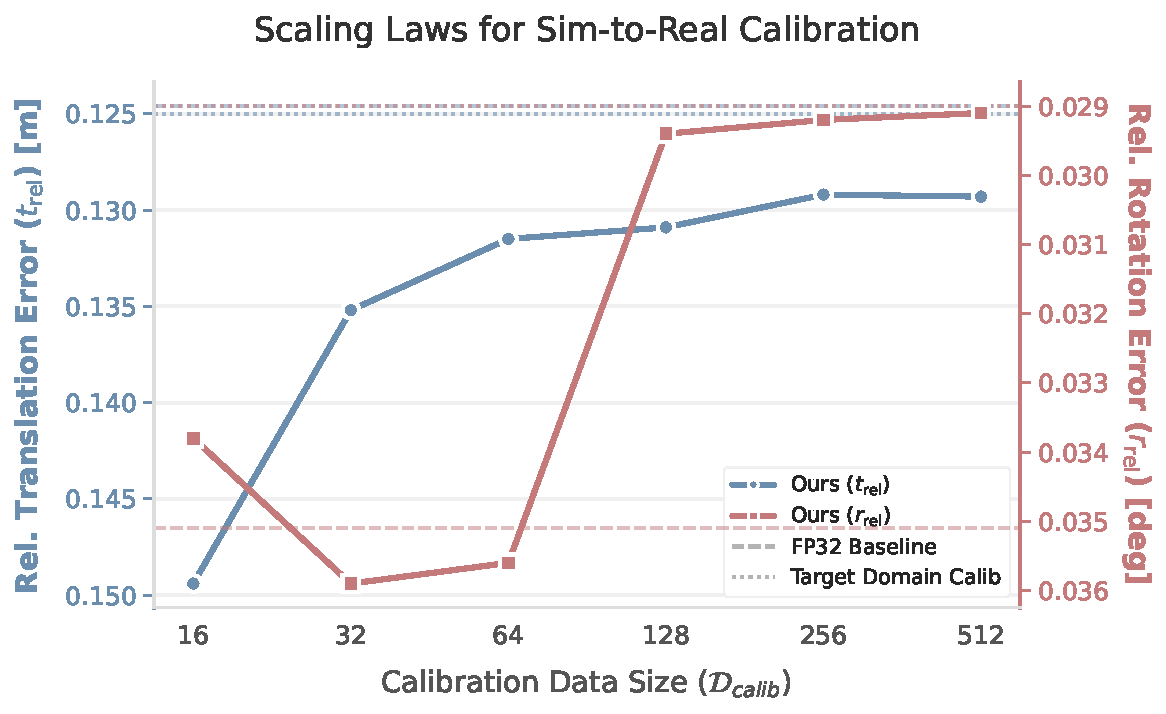
\includegraphics[width=0.8\linewidth]{tex/ch4_quantmacvo/figs/scaling_law_inverted.pdf}
  \captionsetup{font=small}
  \caption{\textbf{Scaling Laws for Sim-to-Real Calibration.} 
    We visualize the quantization performance on real-world datasets as a function of the synthetic calibration data size ($\mathcal{D}_{calib}$). 
    The left and right Y-axes represent relative translation error ($t_{\mathrm{rel}}$) and rotation error ($r_{\mathrm{rel}}$), respectively. Note that the Y-axes are inverted, so that \textit{higher} positions indicate better performance. The curves demonstrate a monotonic performance improvement that saturates around 256 frames.}
    \label{fig:scaling_law_curve}
\end{figure}

To visually analyze the impact of calibration data diversity, we plot quantization error as a function of the number of synthetic calibration frames in \fref{fig:scaling_law_curve}.
The curves reveal a \textit{scaling law} for Sim-to-Real quantization: both translation error (blue) and rotation error (red) decrease monotonically as the calibration set size grows from 16 to 256 frames. The error curves begin to flatten around 128 frames and essentially saturate by 256 frames. At this point, the performance of our method becomes nearly indistinguishable from that of the target-domain calibration baseline. This result suggests that roughly 256 carefully diversified synthetic frames are sufficient to construct a quantization envelope that adequately captures the statistics of established real-world datasets such as KITTI and EuRoC.


% Appendix sections (Ablation Study on Sampling Strategy, Selected Layer List, PTQ Profiling Time) moved to appendix.tex
% 
\section{Ablation Study on Sampling Strategy}
\label{sec:sampling_ablation}

\begin{table*}[h]
    \scriptsize
    \centering
    \captionsetup{font=scriptsize}
    \caption{Ablation Study on Calibration Sampling Strategies. We analyze the impact of different frame selection strategies for constructing the synthetic calibration set. The results demonstrate that our \textbf{Uniform} sampling effectively captures global statistics, outperforming temporally biased methods (Consecutive) and achieving comparable robustness to computation-heavy clustering methods (K-Means) across real-world benchmarks.}
    % \vspace{-.8em}
    \label{tab:quantmacvo:ablation_sample}
    \resizebox{0.8\linewidth}{!}{
    \begin{tabular}{l|c|c|cc|cc|cc|ccc}
        \toprule
        \multirow{2}{*}{\textbf{Sampling Strategy}} & \multirow{2}{*}{\textbf{Description}} &\multirow{2}{*}{\textbf{W/A Bits}} & \multicolumn{2}{c|}{\textbf{TartanAir (Sim)}} & \multicolumn{2}{c|}{\textbf{EuRoC (Real)}} & \multicolumn{2}{c|}{\textbf{KITTI (Real)}} & \multicolumn{2}{c}{\textbf{Avg.}}\\
        &  & & $r_{\mathrm{rel}}$ & $t_{\mathrm{rel}}$ & $r_{\mathrm{rel}}$ & $t_{\mathrm{rel}}$ & $r_{\mathrm{rel}}$ & $t_{\mathrm{rel}}$ & $r_{\mathrm{rel}}$ & $t_{\mathrm{rel}}$ \\
        \midrule
        \rowcolor{gray!5} \multicolumn{2}{l|}{Baseline}&FP32 / FP32 & .0790 & .2670 & .0028 & .0468 & .0164 & .0360 & .0351 & .1246 \\
        \midrule
        \multicolumn{10}{l}{\textit{Quantized (W8A8) with different calibration sampling:}} \\
        Consecutive & \footnotesize{Sequential frames (Temporal Bias)} &INT8 / INT8 & .1250 & .4520 & .0045 & .0850 & .0210 & .0520 & .0541 & .2098 \\
        Random & \footnotesize{Random selection} &INT8 / INT8 & .0811 & .2938 & .0029 & .0487 & .0162 &.0368  & .0359 & .1352 \\
        K-Means & \footnotesize{Feature clustering (Diversity)} &INT8 / INT8 & .0730 & .2676 & .0028 & .0475 & .0161 & .0363 & .0328 & .1250 \\
        \midrule
        \rowcolor{gray!20} Uniform & \footnotesize{Uniform sampling (same interval)} &INT8 / INT8 & .0720 & .2630 & .0029 & .0490 & .0161 & .0369 & .0325 & .1240\\
        \bottomrule
    \end{tabular}
    }
    \label{tab:quantmacvo:calib_sample}
\end{table*}

To determine the suitable strategy for constructing the global calibration set $\mathcal{D}_{calib}$, we evaluate four sampling protocols: \textit{Consecutive} (sequential frames), \textit{Random}, \textit{K-Means} (feature clustering for diversity), and Uniform sampling. As presented in \tref{tab:quantmacvo:ablation_sample}, the sampling strategy fundamentally determines the quantization robustness. The \textit{Consecutive} strategy suffers from severe degradation, yielding the highest average relative translation error. This confirms that calibration sets dominated by temporally correlated frames fail to capture the long-tail distribution of the domain, leading to overfitting on local statistics. While \textit{K-Means} clustering effectively maximizes data diversity and recovers performance, it incurs significant computational overhead for feature extraction and clustering. In contrast, Uniform strategy achieves comparable overall performance, slightly outperforming K-Means.
    
This result empirically validates that simple uniform sampling over diverse synthetic sequences is sufficient to approximate the global ``quantization envelope.'' It breaks temporal correlations and covers extreme motion dynamics without the computational cost of complex clustering, making it the most practical choice for efficient Sim-to-Real calibration.


\section{Selected Layer List}
\label{sec:selected_layers}

% Selected quantized operators by architectural component. Preamble: \usepackage{booktabs}
\begin{table}[h]
  \centering
  \caption{Selected layers for Hadamard rotation in the QuantMAC-VO front-end (depth 12; 28 layers are selected). All remaining layers are quantized with SmoothQuant.}

  \label{tab:quantmacvo:selected_layers}
  \resizebox{0.5\linewidth}{!}{
  \begin{tabular}{@{}r p{0.92\columnwidth}@{}}
  \toprule
  \multicolumn{2}{@{}l@{}}{\textbf{Context Encoder -- MLP}} \\
  \midrule
  19 & \ttfamily svt.blocks.1.1.mlp.fc1 \\
  \midrule
  \multicolumn{2}{@{}l@{}}{\textbf{Memory Encoder -- Feature encoder MLP}} \\
  \midrule
  20 & \ttfamily feat\_encoder.svt.blocks.0.0.mlp.fc1 \\
  21 & \ttfamily feat\_encoder.svt.blocks.0.0.mlp.fc2 \\
  \midrule
  \multicolumn{2}{@{}l@{}}{\textbf{Memory Encoder -- Patch embedding / attention context projection}} \\
  \midrule
  22 & \ttfamily patch\_embed.proj.4 \\
  23 & \ttfamily vertical\_encoder\_layers.0.local\_block.attn.context\_proj \\
  24 & \ttfamily vertical\_encoder\_layers.0.global\_block.attn.context\_proj \\
  25 & \ttfamily vertical\_encoder\_layers.1.local\_block.attn.context\_proj \\
  26 & \ttfamily vertical\_encoder\_layers.1.global\_block.attn.context\_proj \\
  27 & \ttfamily vertical\_encoder\_layers.2.local\_block.attn.context\_proj \\
  28 & \ttfamily vertical\_encoder\_layers.2.global\_block.attn.context\_proj \\
  \midrule

  \multicolumn{2}{@{}l@{}}{\textbf{Memory Decoder -- Covariance update \& GRU gating}} \\
  \midrule
  1  & \ttfamily cov\_update.cov\_head.conv2 \\
  5  & \ttfamily cov\_update.gru.convq2 \\
  7  & \ttfamily cov\_update.gru.convq1 \\
  9  & \ttfamily cov\_update.gru.convz1 \\
  10 & \ttfamily cov\_update.gru.convr1 \\
  11 & \ttfamily cov\_update.gru.convz2 \\
  12 & \ttfamily cov\_update.gru.convr2 \\
  \midrule
  \multicolumn{2}{@{}l@{}}{\textbf{Memory Decoder -- Encoder / Flow head / Aggregation}} \\
  \midrule
  2  & \ttfamily update\_block.flow\_head.conv2 \\
  3  & \ttfamily update\_block.encoder.conv \\
  13 & \ttfamily update\_block.encoder.convf2 \\
  8  & \ttfamily update\_block.aggregator.to\_v \\
  \midrule
  \multicolumn{2}{@{}l@{}}{\textbf{Memory Decoder -- GRU \& projection}} \\
  \midrule
  4  & \ttfamily update\_block.gru.convq2 \\
  6  & \ttfamily update\_block.gru.convq1 \\
  14 & \ttfamily update\_block.gru.convz1 \\
  15 & \ttfamily update\_block.gru.convr1 \\
  16 & \ttfamily update\_block.gru.convz2 \\
  17 & \ttfamily update\_block.gru.convr2 \\
  18 & \ttfamily proj \\
  \bottomrule
  \end{tabular}}
\end{table}


\section{PTQ Profiling Time}
\label{sec:ptq_profiling}

In the Methodology section, we highlight a key limitation of layer-wise sensitivity profiling: it substantially increases PTQ profiling time. Because layer-wise profiling quantizes and evaluates one layer at a time, it requires repeated forward passes that scale linearly with the number of layers. In contrast, our method estimates layer importance using only full-precision forward passes over the analysis set, resulting in much lower profiling cost. Our method completes profiling in under one minute and is 460$\times$ faster than the layer-wise baseline on an RTX 3090 Ti using the same analysis set (32 samples).

\begin{table}[htbp]
\centering
\captionsetup{font=small}
\caption{PTQ profiling time (min) comparison between layer-wise sensitivity method and ours.}
\begin{tabular}{lcc}
\toprule
 & Layer-wise & Ours \\
\midrule
Time (min) & 227.12 & 0.48 (460$\times$) \\
\bottomrule
\end{tabular}
\label{tab:quantmacvo:profiling_time}
\end{table}



\section{Conclusion and Discussion}
\label{sec:quantmacvo_conclusion}

This chapter presents QuantMAC-VO, a post-training quantization framework tailored for learning-based visual odometry with metrics-aware covariance. By leveraging a kurtosis-guided hybrid quantization scheme and a Sim-to-Real calibration strategy, the method effectively mitigates the impact of non-stationary distributions and outlier activations inherent in VO tasks. We empirically demonstrated a scaling law where synthetic calibration diversity directly translates to real-world robustness, enabling a $1.42\times$ to $2.89\times$ speedup on the NVIDIA Jetson Thor platform with comparable accuracy.

A primary limitation is that the backend optimization still relies on floating-point arithmetic (albeit with explicit scaling) to preserve numerical stability, preventing a fully integer-only pipeline. Future work will focus on exploring fully quantized graph optimization to eliminate remaining floating-point overhead, and investigating lower-bit quantization (e.g., W4A4) to further reduce memory footprint for deployment on ultra-low-power microcontrollers.

Together with MAC-VO (Chapter~\ref{chapter:macvo}), this chapter completes Part~I of the thesis: metrics-aware visual uncertainty can be learned, integrated into a full VO pipeline, and efficiently deployed on edge hardware while preserving both pose accuracy and uncertainty quality.
